
\chapter{}

\section{Analisis de los requisitos}
    
    \subsection{Modelo conceptual}

A continuación podemos ver los principales conceptos que comprende el sistema y cómo se relacionan. De la interfaz y sus conceptos hablaremos en el diseño de la interfaz.


 \begin{figure}[H] %con el [H] le obligamos a situar aquí la figura
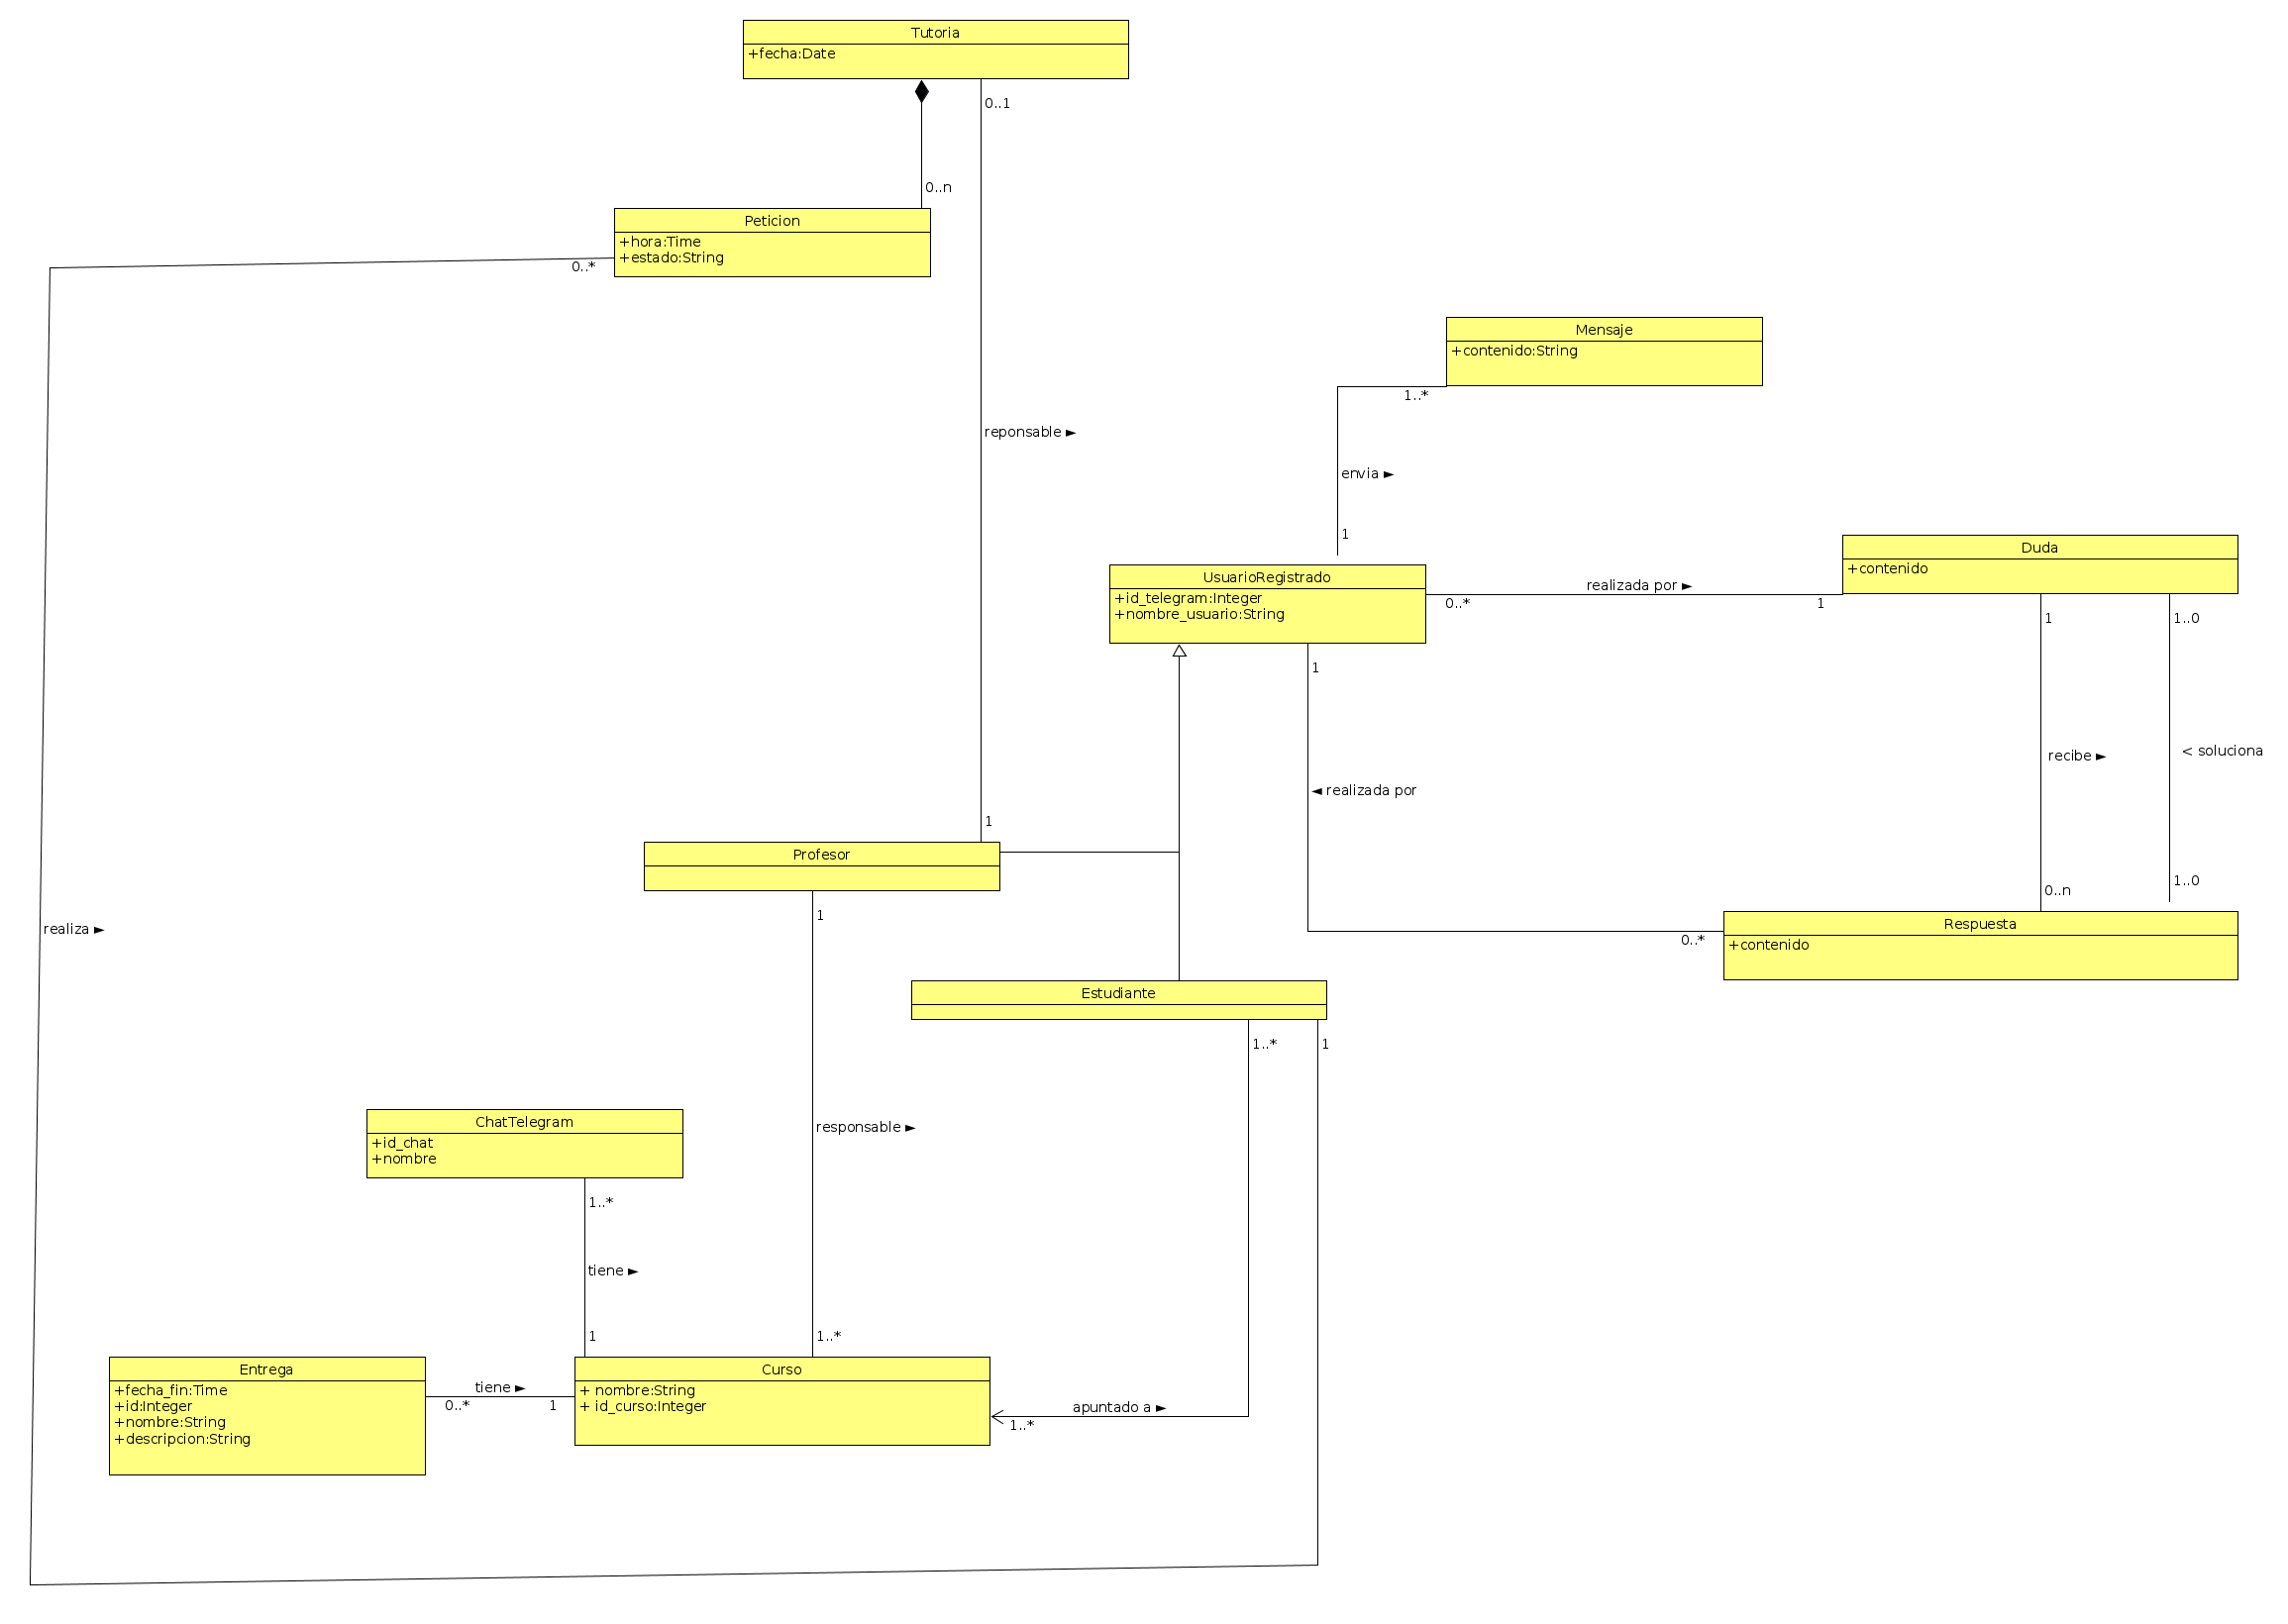
\includegraphics[width=1.1\textwidth, right]{imagenes/diagramas/diagrama_conceptual.png}  %el parámetro scale permite agrandar o achicar la imagen. En el nombre de archivo puede especificar directorios
\caption{Diagrama conceptual del sistema}\label{figura197}
\end{figure}


Presenta cierto parecido con el diagrama de casos de uso: profesor y estudiante heredan de usuario registrado que tienen relación con las dudas, profesor responsable de las tutorías y el estudiante realiza peticiones a éstas.

\subsection{Diagramas secuencia}

La meta buscada en esta sección es mostrar las interacciones entre los objetos que provoca la realización de algunos de los CUs más importantes por parte de los actores. Ahora mismo hay una clase \enquote*{pradobot} que hace de mediadora entre el usuario y el resto de clases del sistema. Esta clase dirime qué es lo que quiere el usuario y lleva a cabo las interacciones necesarias con el resto de clases para cumplir el objetivo del usuario. Todas estas operaciones exigidas por el usuario se traducirán en interfaces cuyo diseño se tratará en la sección de diseño interacción usuario.


\begin{figure}[H] %con el [H] le obligamos a situar aquí la figura
\centering
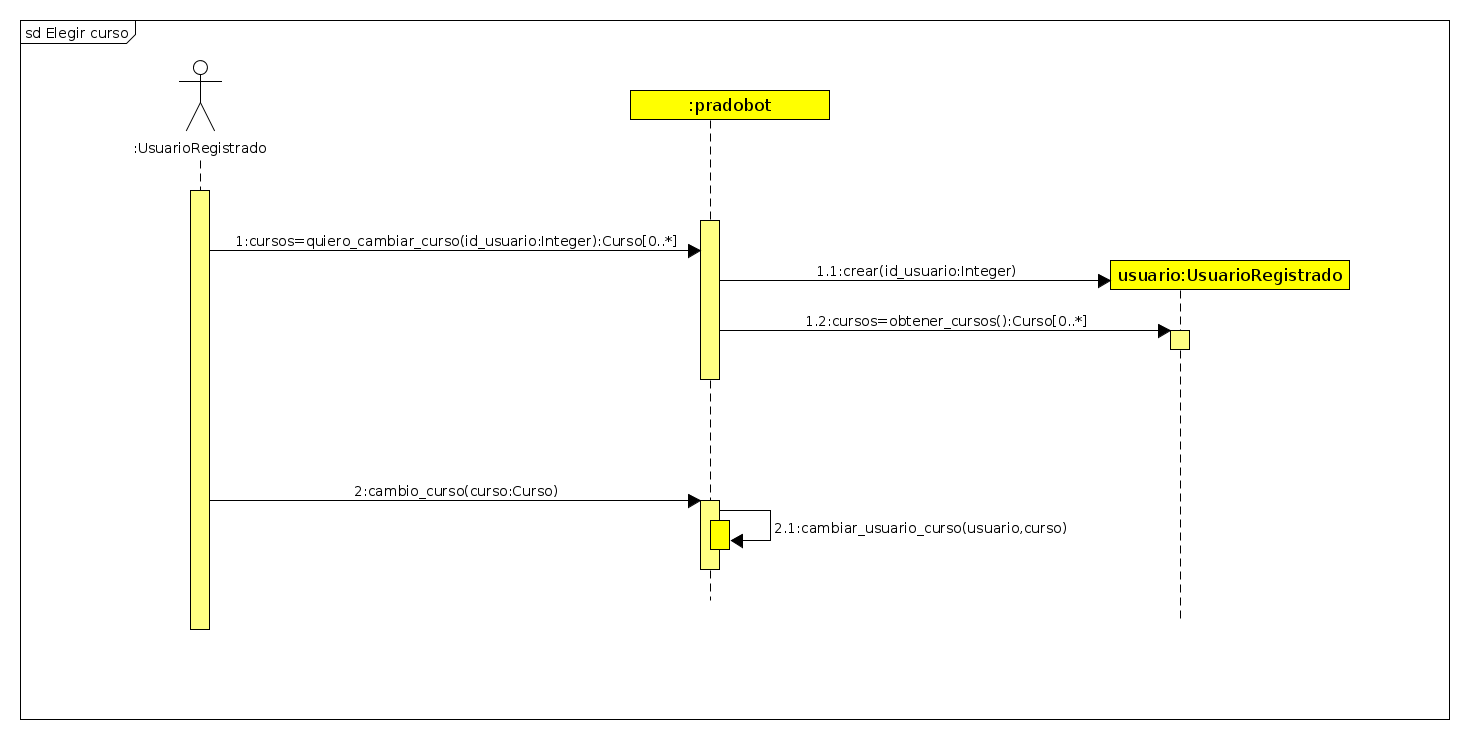
\includegraphics[scale=0.3]{imagenes/diagramas/secuencia/analisis/elegir_curso.png}  %el parámetro scale permite agrandar o achicar la imagen. En el nombre de archivo puede especificar directorios

\caption{DS: Cambiar curso (CU-1.4) }\label{figura62}

\end{figure}

\begin{figure}[H] %con el [H] le obligamos a situar aquí la figura
\centering
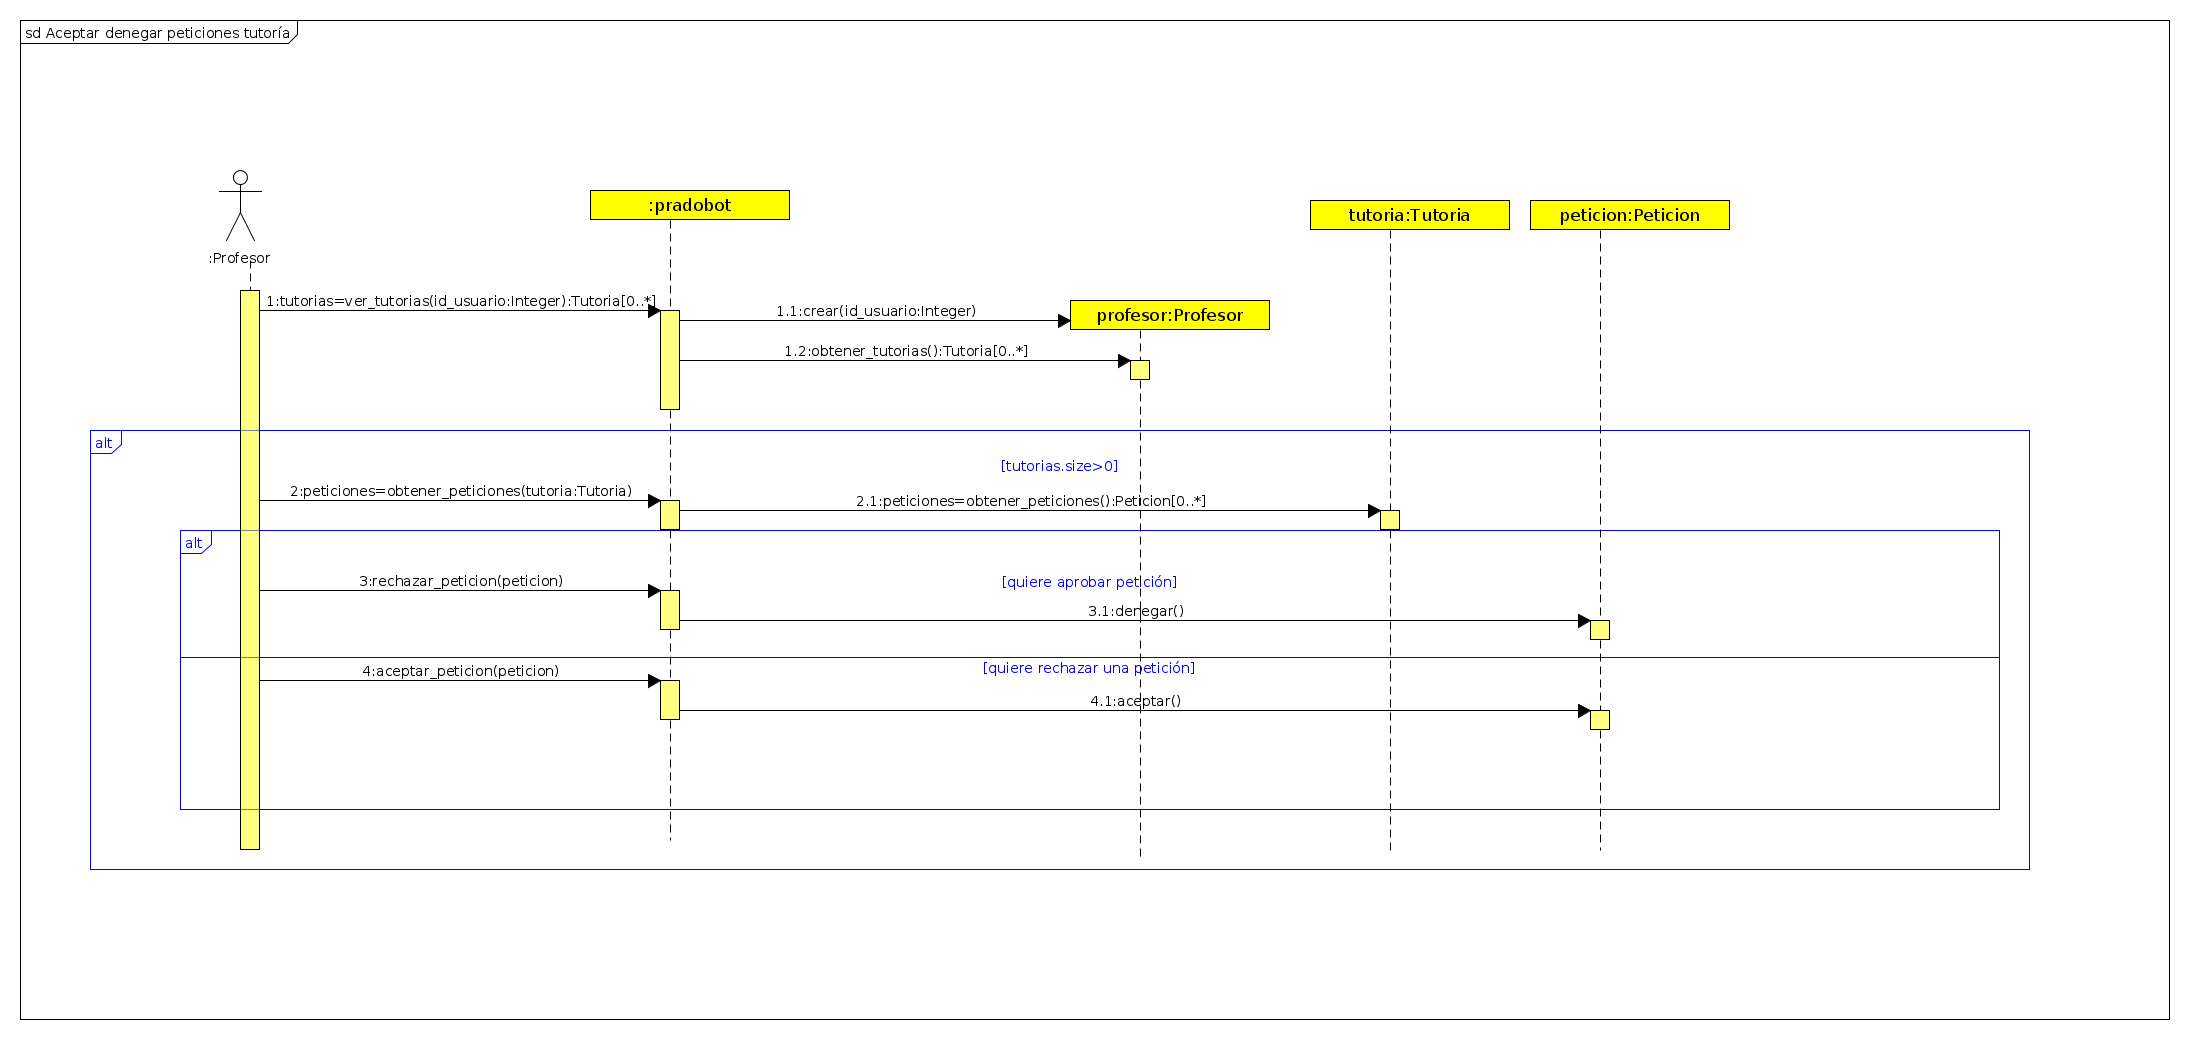
\includegraphics[scale=0.2]{imagenes/diagramas/secuencia/analisis/aceptar_denegar_peticion.png}  %el parámetro scale permite agrandar o achicar la imagen. En el nombre de archivo puede especificar directorios

\caption{DS: Aceptar denegar peticiones (CU-4.4, CU-4.5) }\label{figura72}

\end{figure}

\begin{figure}[H] %con el [H] le obligamos a situar aquí la figura
\centering
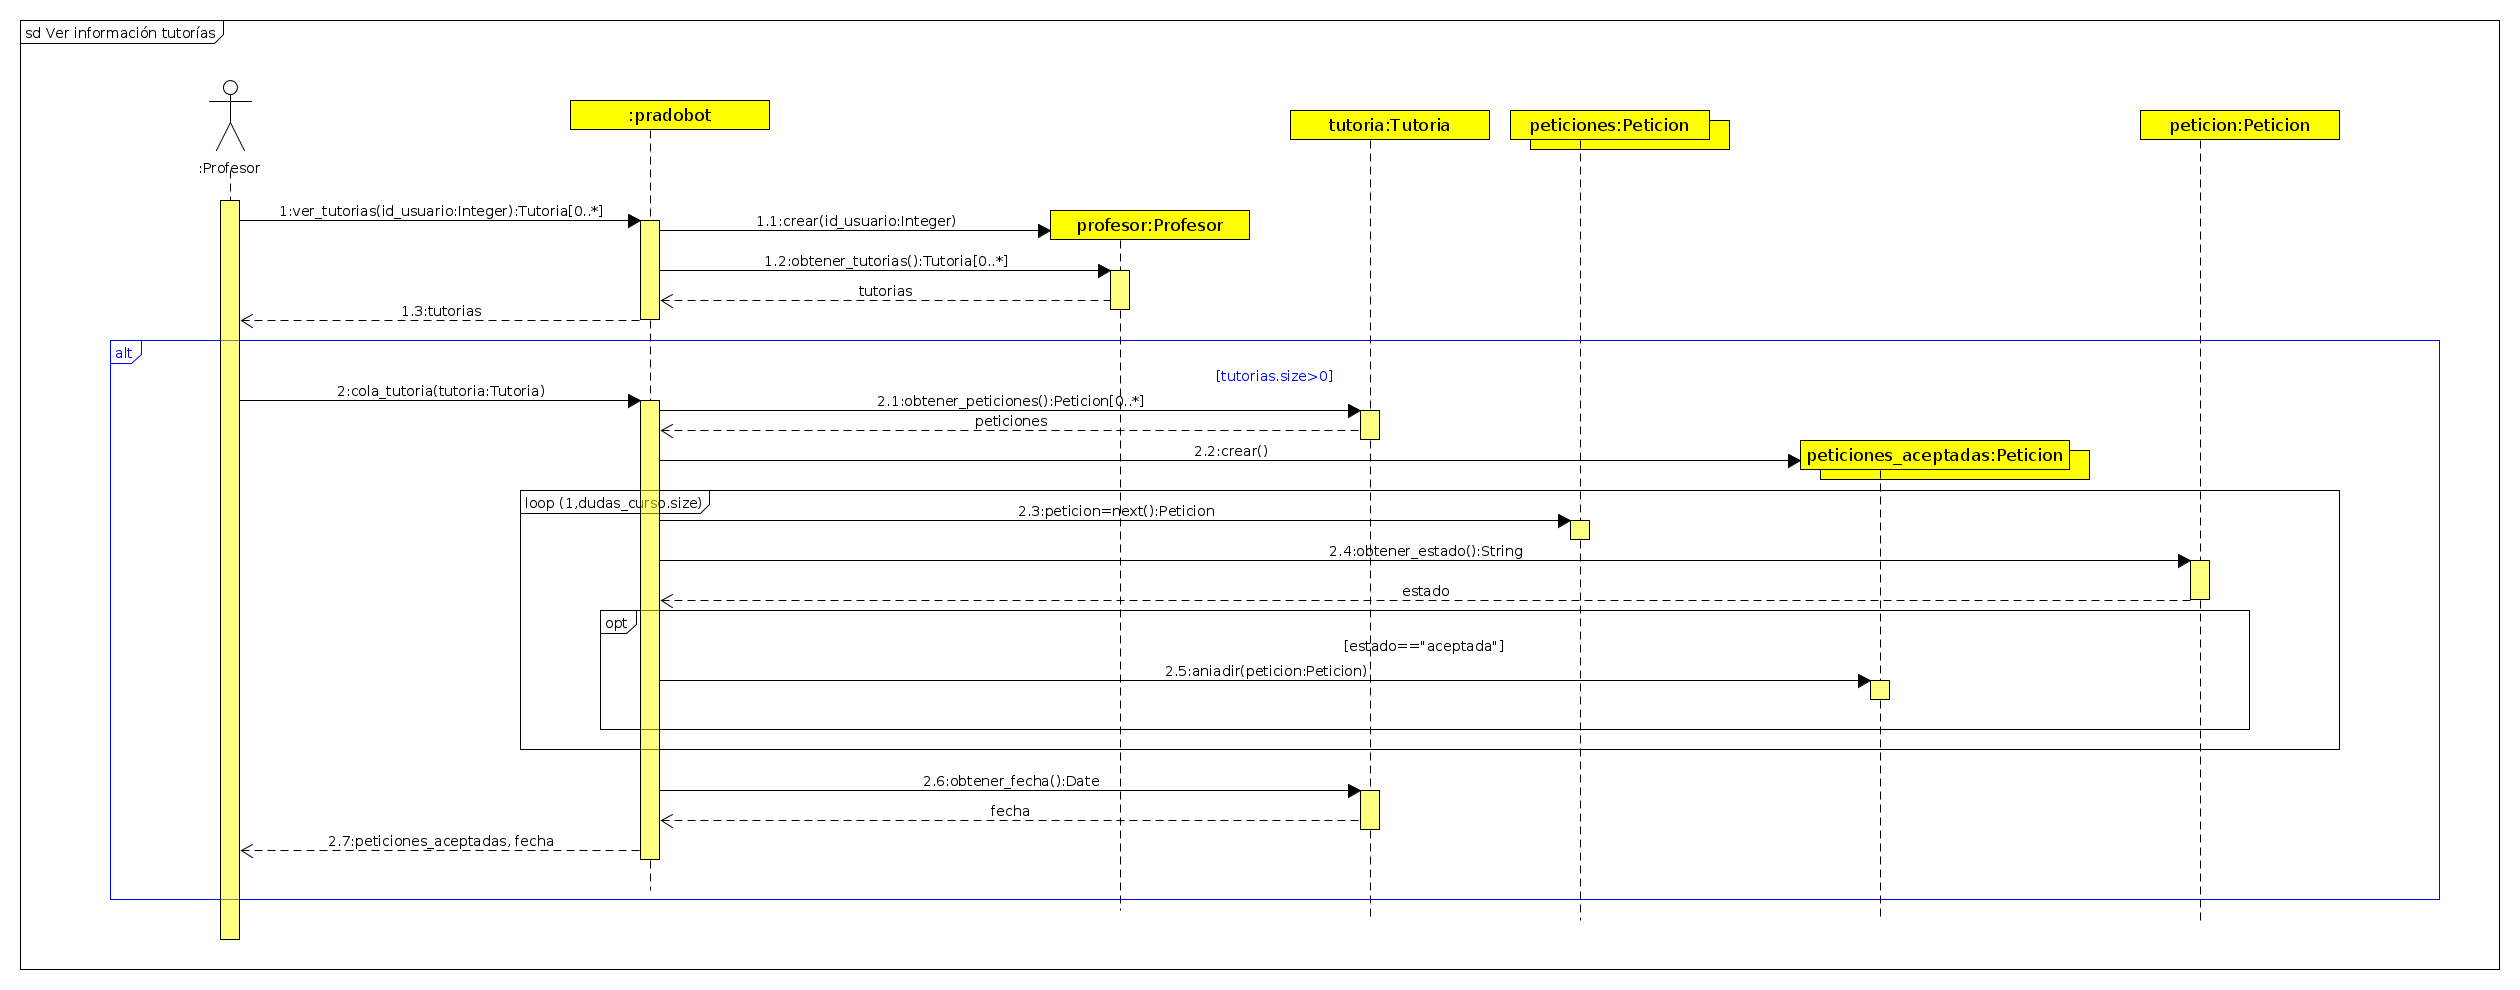
\includegraphics[width=1.3\textwidth]{imagenes/diagramas/secuencia/analisis/ver_informacion_tutoria.png}  %el parámetro scale permite agrandar o achicar la imagen. En el nombre de archivo puede especificar directorios

\caption{DS: Ver información tutoria (CU-4.6) }\label{figura77}

\end{figure}

\begin{figure}[H] %con el [H] le obligamos a situar aquí la figura
\centering
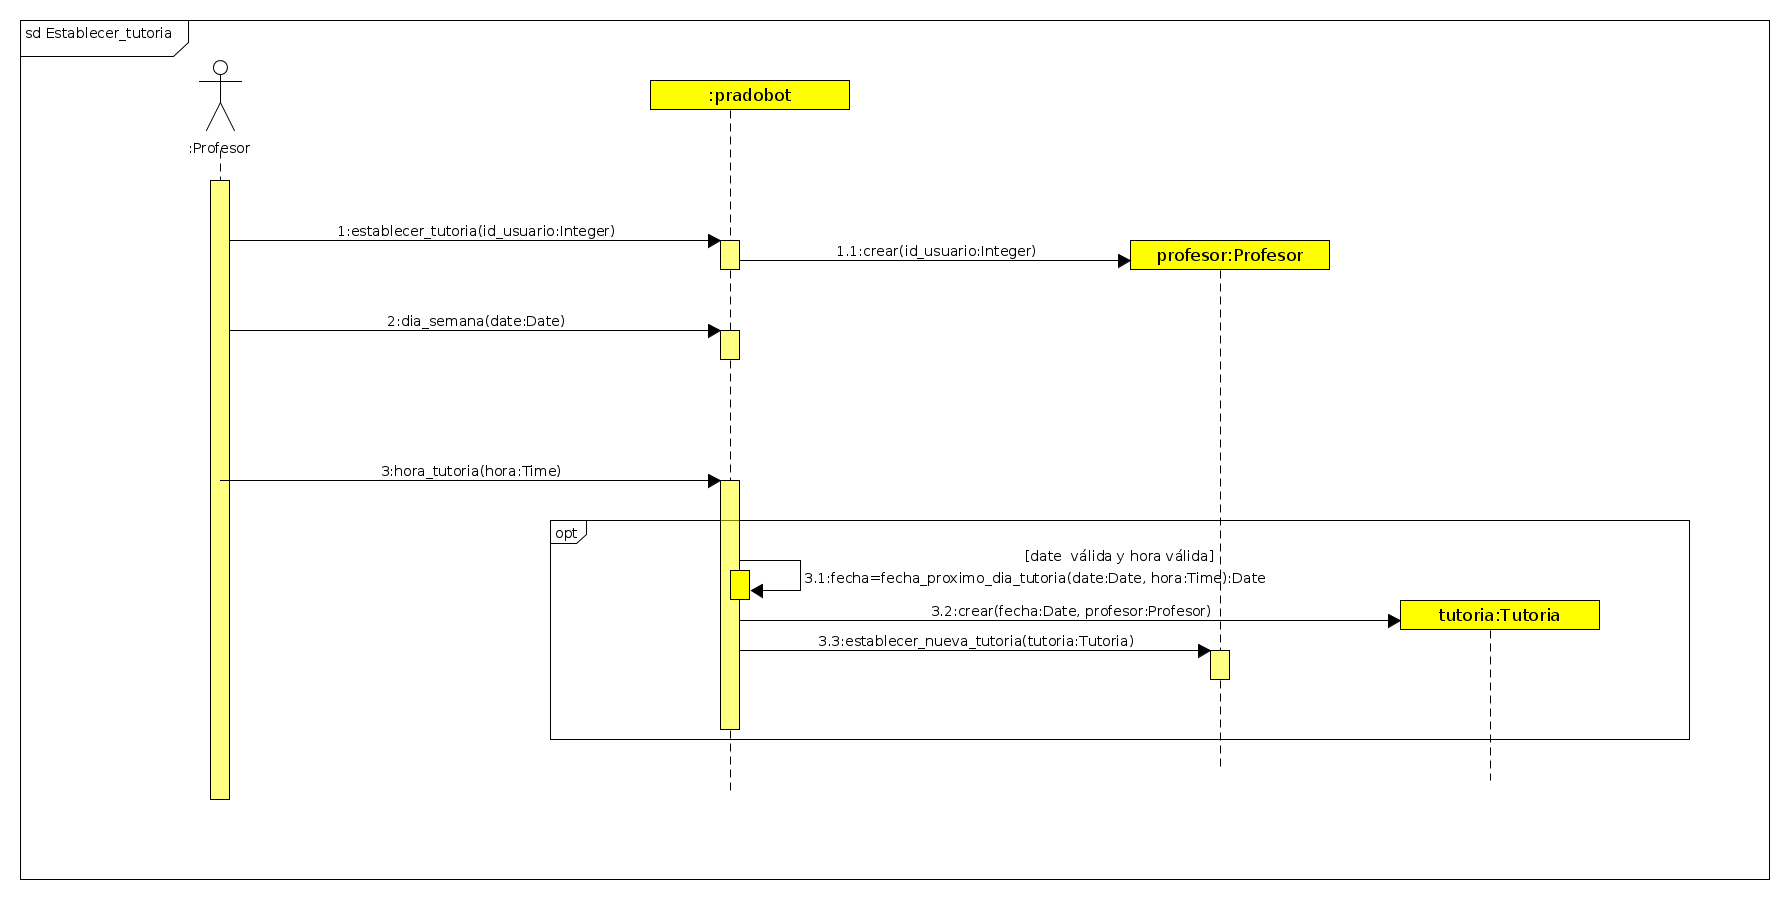
\includegraphics[width=1.2\textwidth, right]{imagenes/diagramas/secuencia/analisis/establecer_tutoria.png}  %el parámetro scale permite agrandar o achicar la imagen. En el nombre de archivo puede especificar directorios

\caption{DS: Establecer tutoría (CU-4.1) }\label{figura211}

\end{figure}

\begin{figure}[H] %con el [H] le obligamos a situar aquí la figura
\centering
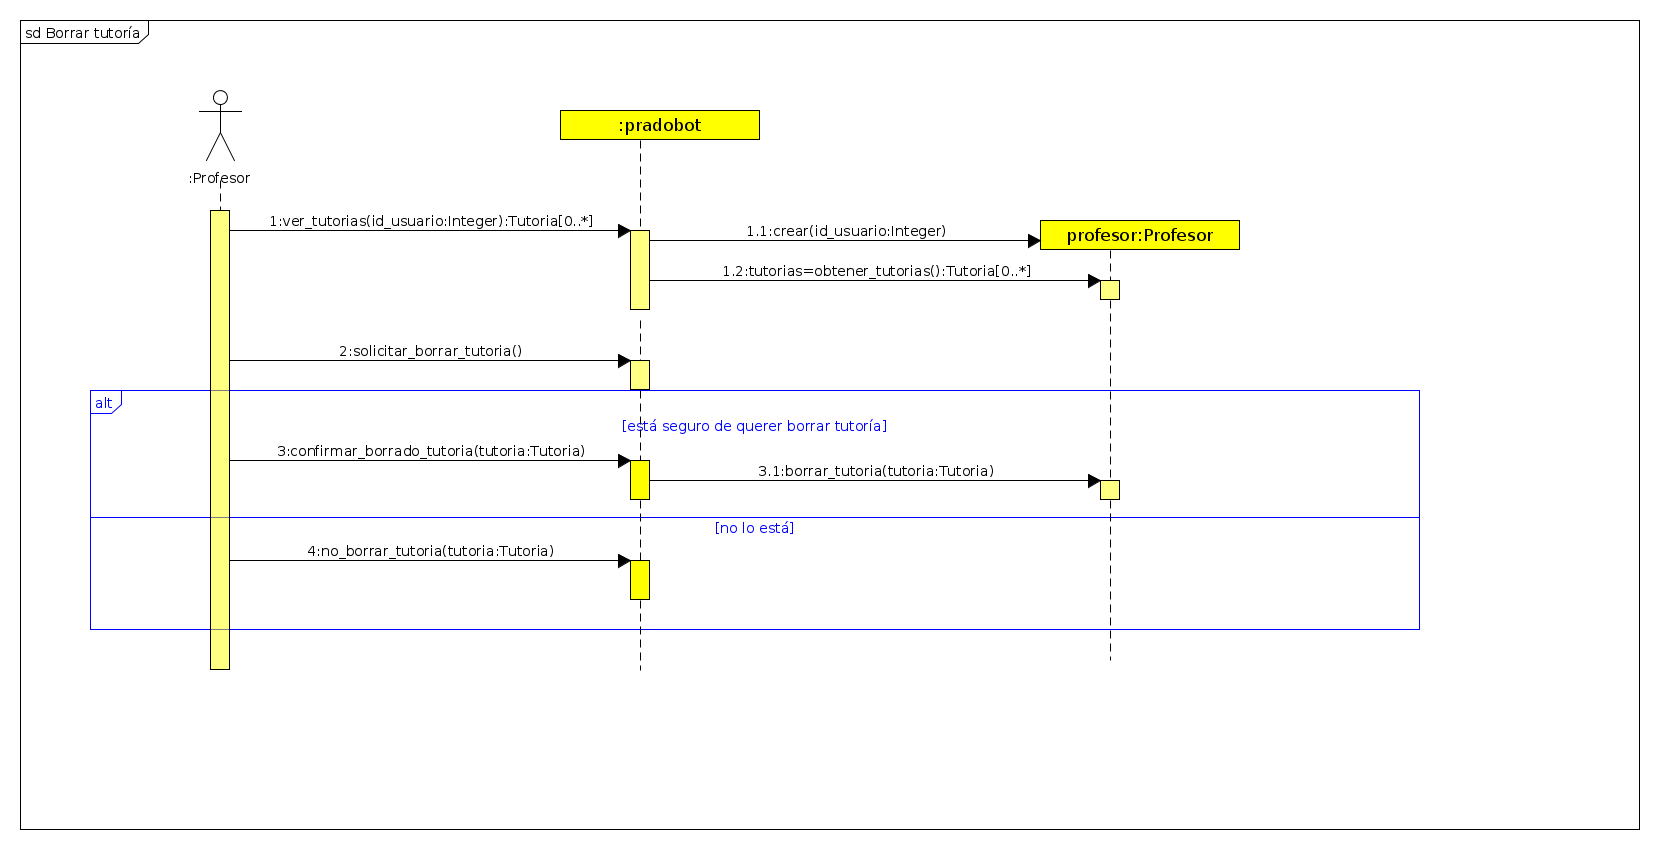
\includegraphics[scale=0.27]{imagenes/diagramas/secuencia/analisis/borrar_tutoria.png}  %el parámetro scale permite agrandar o achicar la imagen. En el nombre de archivo puede especificar directorios

\caption{DS: Borrar tutoría (CU-4.2) }\label{figura78}

\end{figure}

\begin{figure}[H] %con el [H] le obligamos a situar aquí la figura
\centering
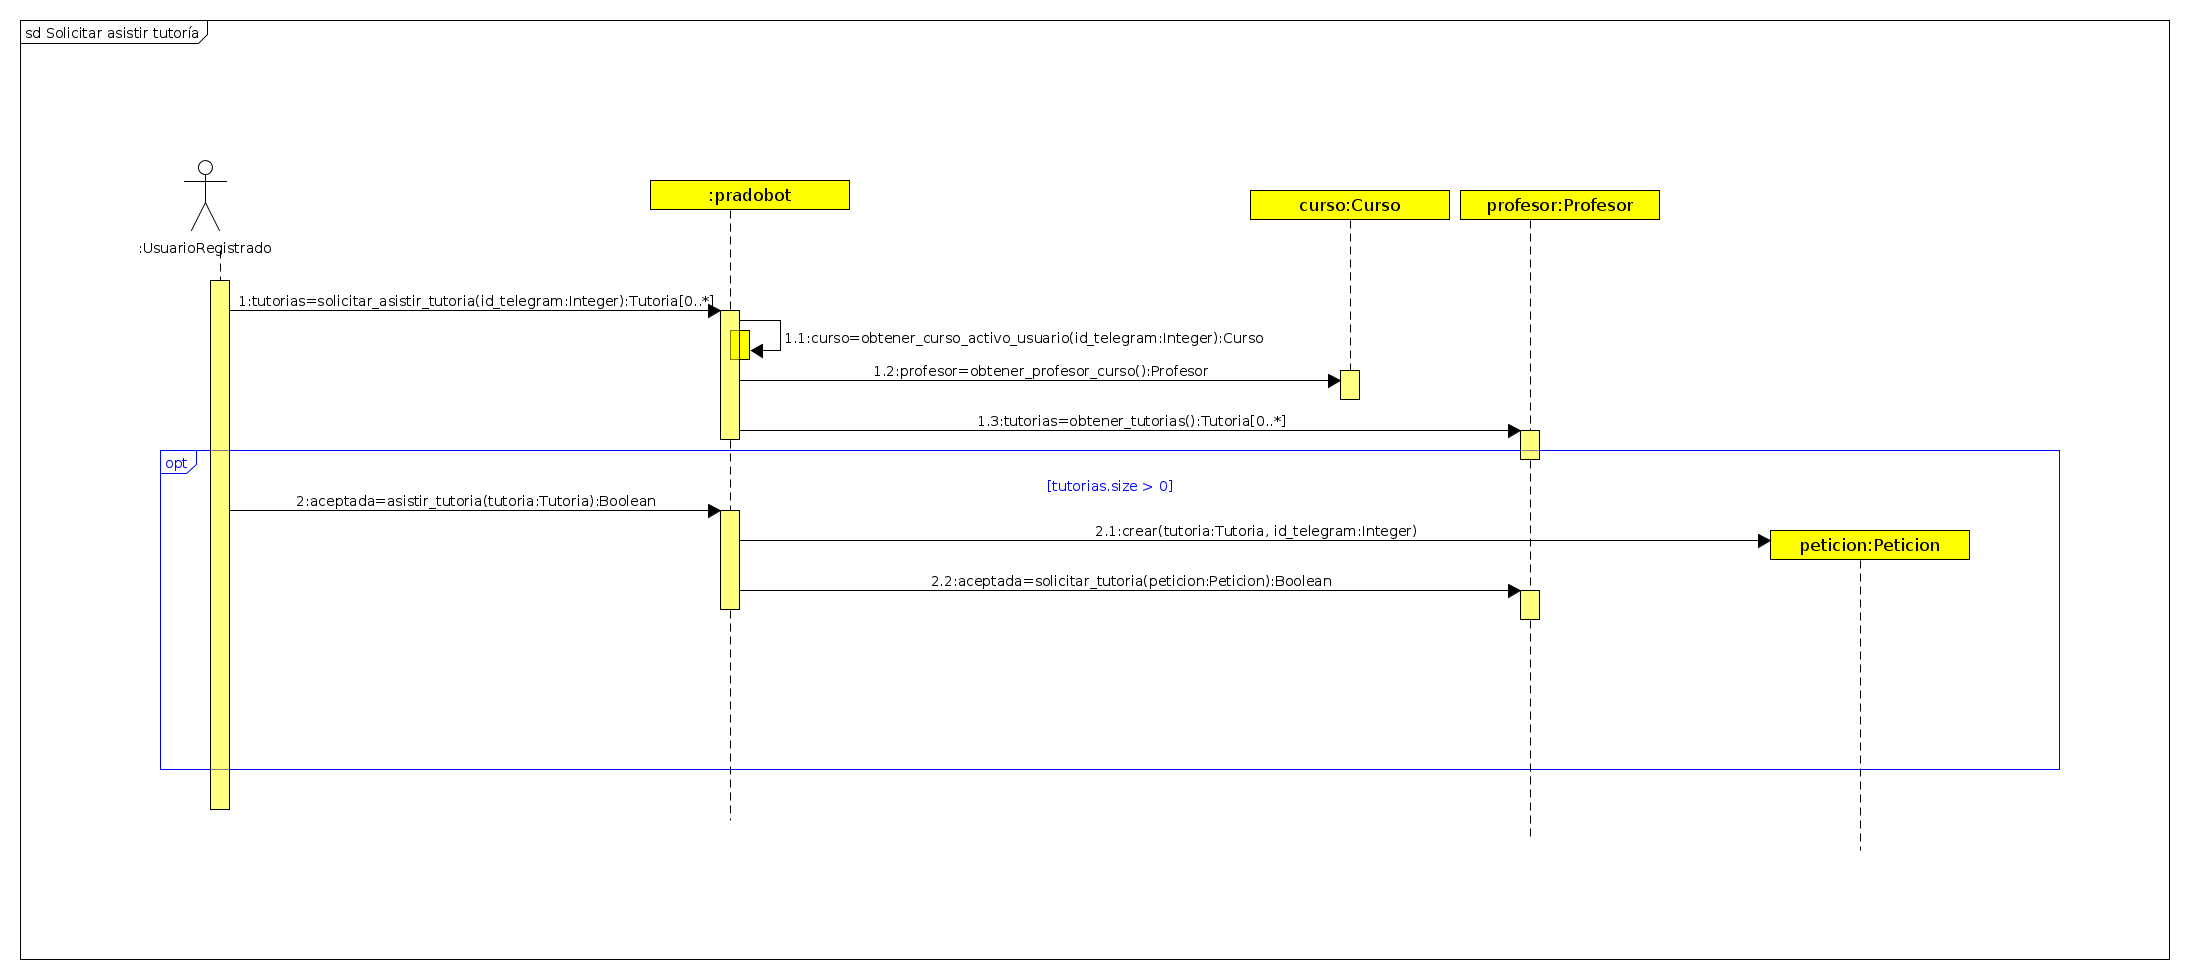
\includegraphics[scale=0.22]{imagenes/diagramas/secuencia/analisis/asistir_tutoria.png}  %el parámetro scale permite agrandar o achicar la imagen. En el nombre de archivo puede especificar directorios

\caption{DS: Solicitar asistir tutoría (CU-4.3) }\label{figura79}

\end{figure}

\begin{figure}[H] %con el [H] le obligamos a situar aquí la figura
\centering
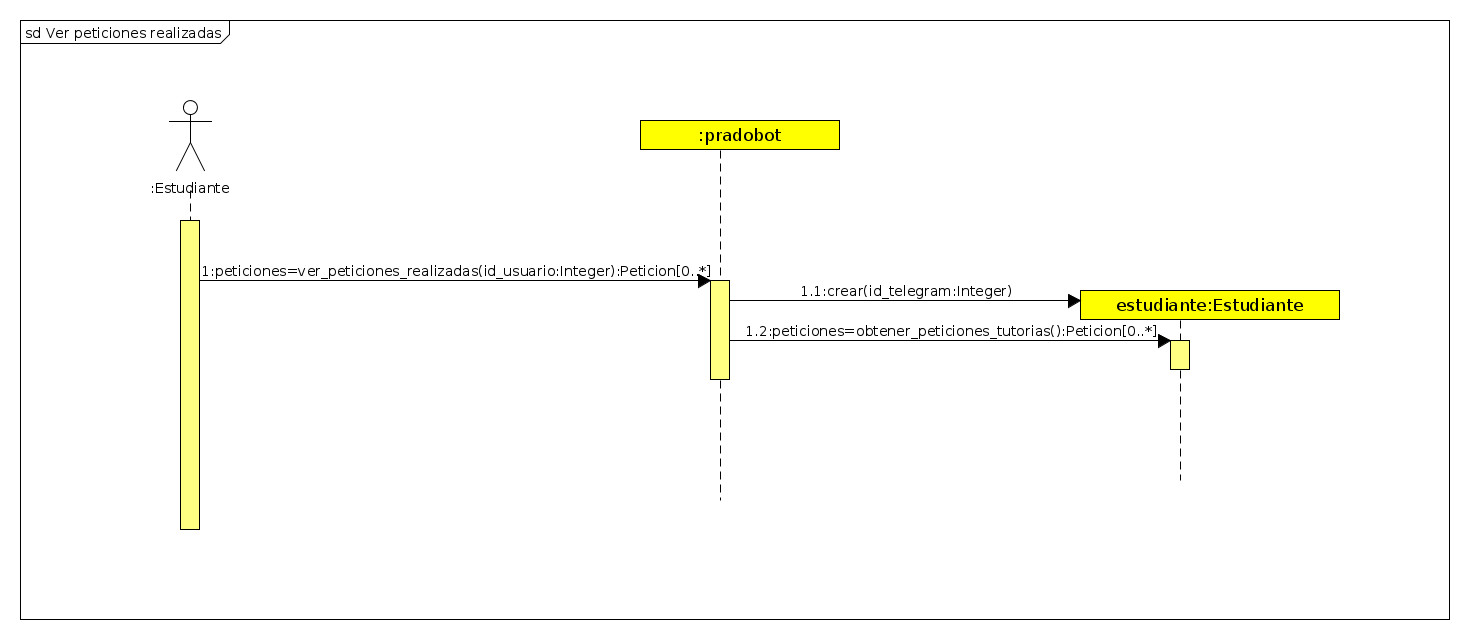
\includegraphics[scale=0.3]{imagenes/diagramas/secuencia/analisis/ver_peticiones_realizadas.png}  %el parámetro scale permite agrandar o achicar la imagen. En el nombre de archivo puede especificar directorios

\caption{DS: Ver solicitudes realizadas (CU-4.7) }\label{figura80}

\end{figure}


\begin{figure}[H] %con el [H] le obligamos a situar aquí la figura
\centering
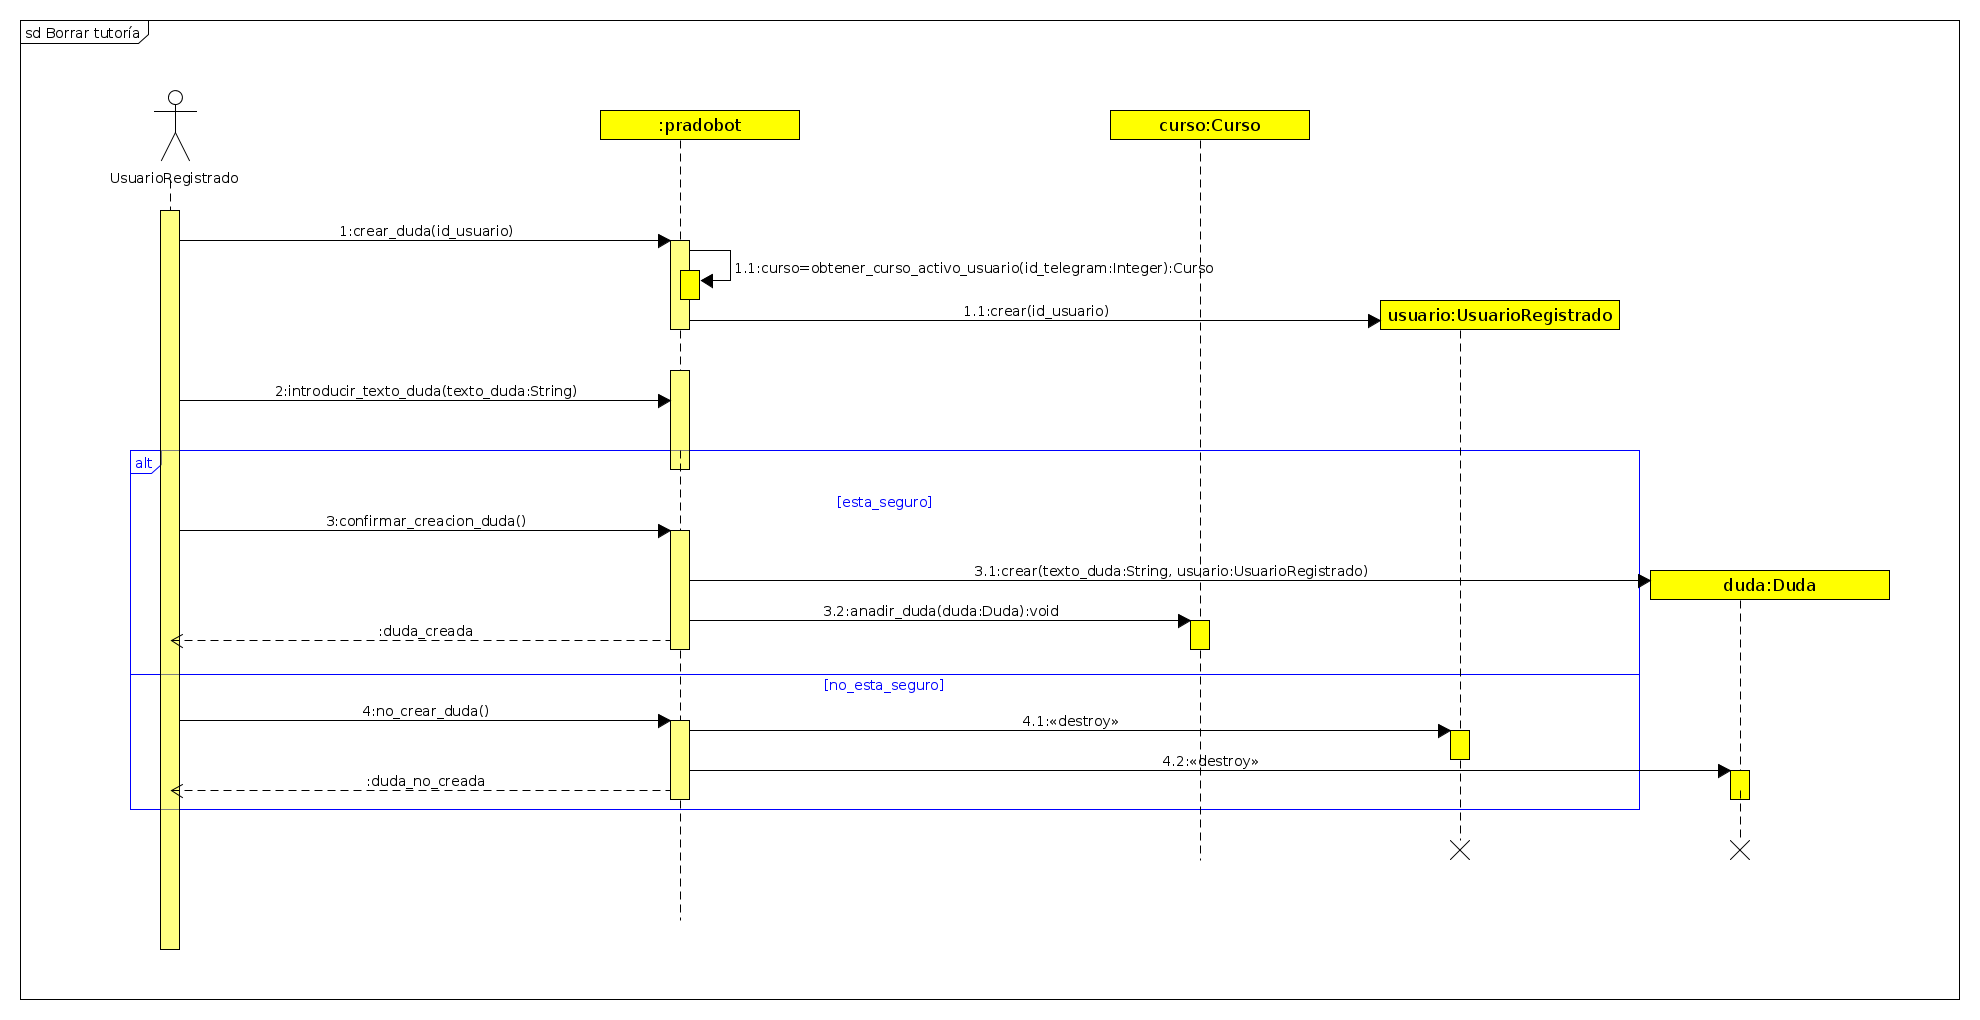
\includegraphics[scale=0.22]{imagenes/diagramas/secuencia/analisis/crear_duda.png}  %el parámetro scale permite agrandar o achicar la imagen. En el nombre de archivo puede especificar directorios

\caption{DS: Crear duda (CU-5.1) }\label{figura81}

\end{figure}

\begin{figure}[H] %con el [H] le obligamos a situar aquí la figura
\centering
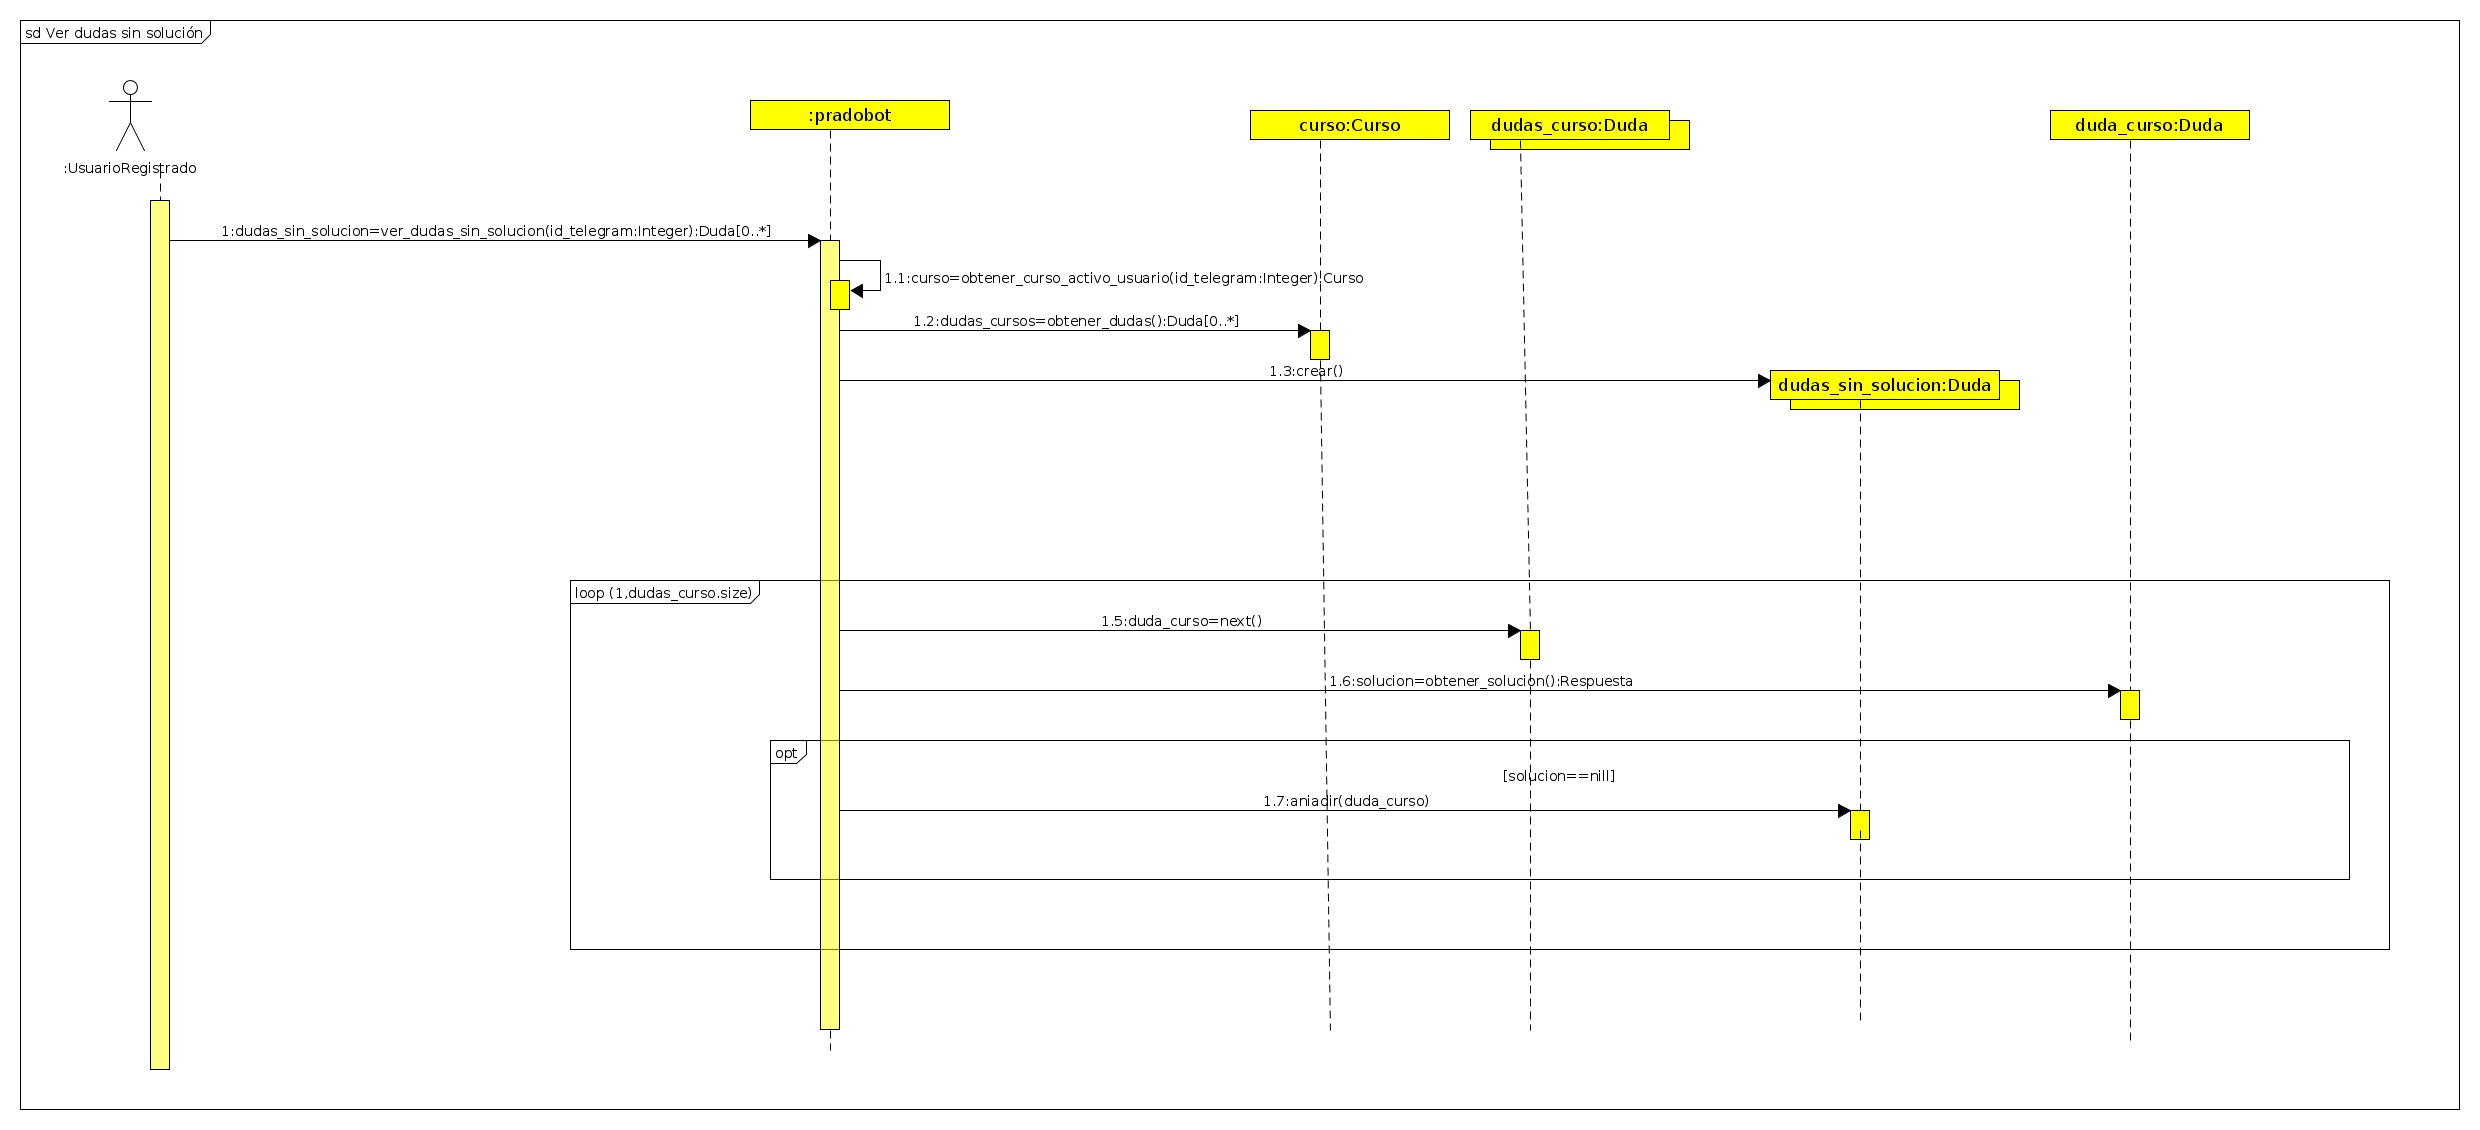
\includegraphics[scale=0.17]{imagenes/diagramas/secuencia/analisis/ver_dudas_sin_solucion.png}  %el parámetro scale permite agrandar o achicar la imagen. En el nombre de archivo puede especificar directorios

\caption{DS: Ver dudas sin solución (CU-5.2) }\label{figura83}

\end{figure}

\begin{figure}[H] %con el [H] le obligamos a situar aquí la figura
\centering
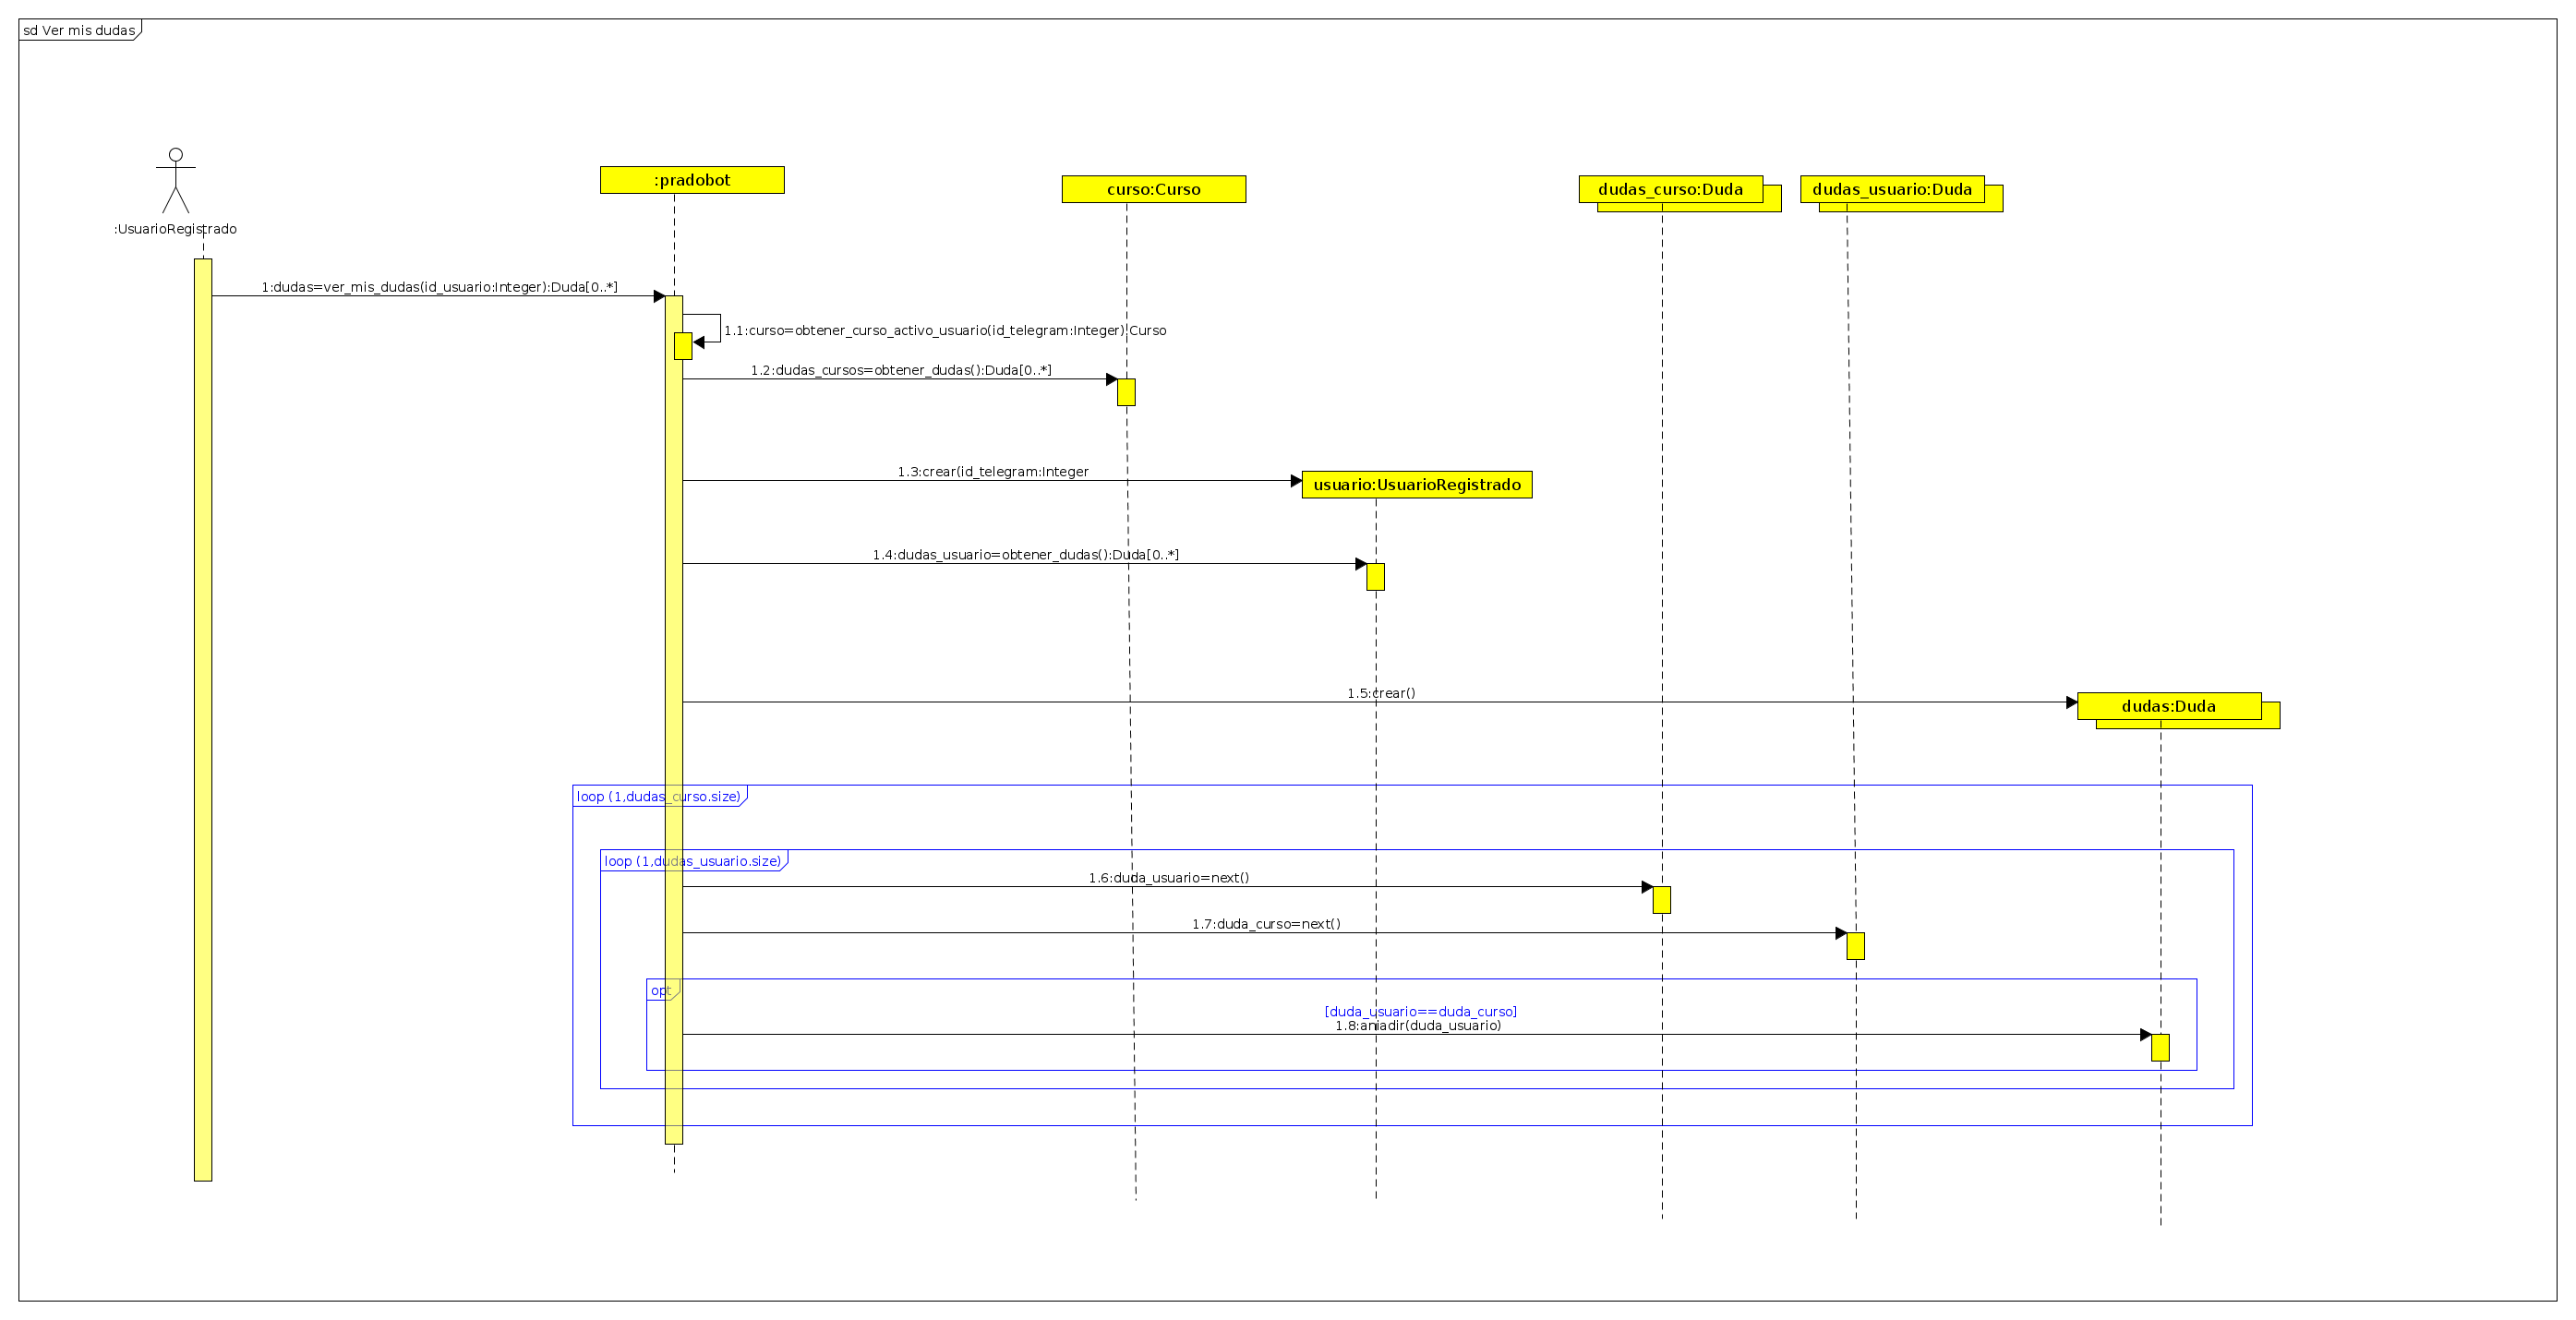
\includegraphics[scale=0.18]{imagenes/diagramas/secuencia/analisis/ver_mis_dudas.png}  %el parámetro scale permite agrandar o achicar la imagen. En el nombre de archivo puede especificar directorios

\caption{DS: Ver mis dudas (CU-5.3) }\label{figura84}

\end{figure}

\begin{figure}[H] %con el [H] le obligamos a situar aquí la figura
\centering
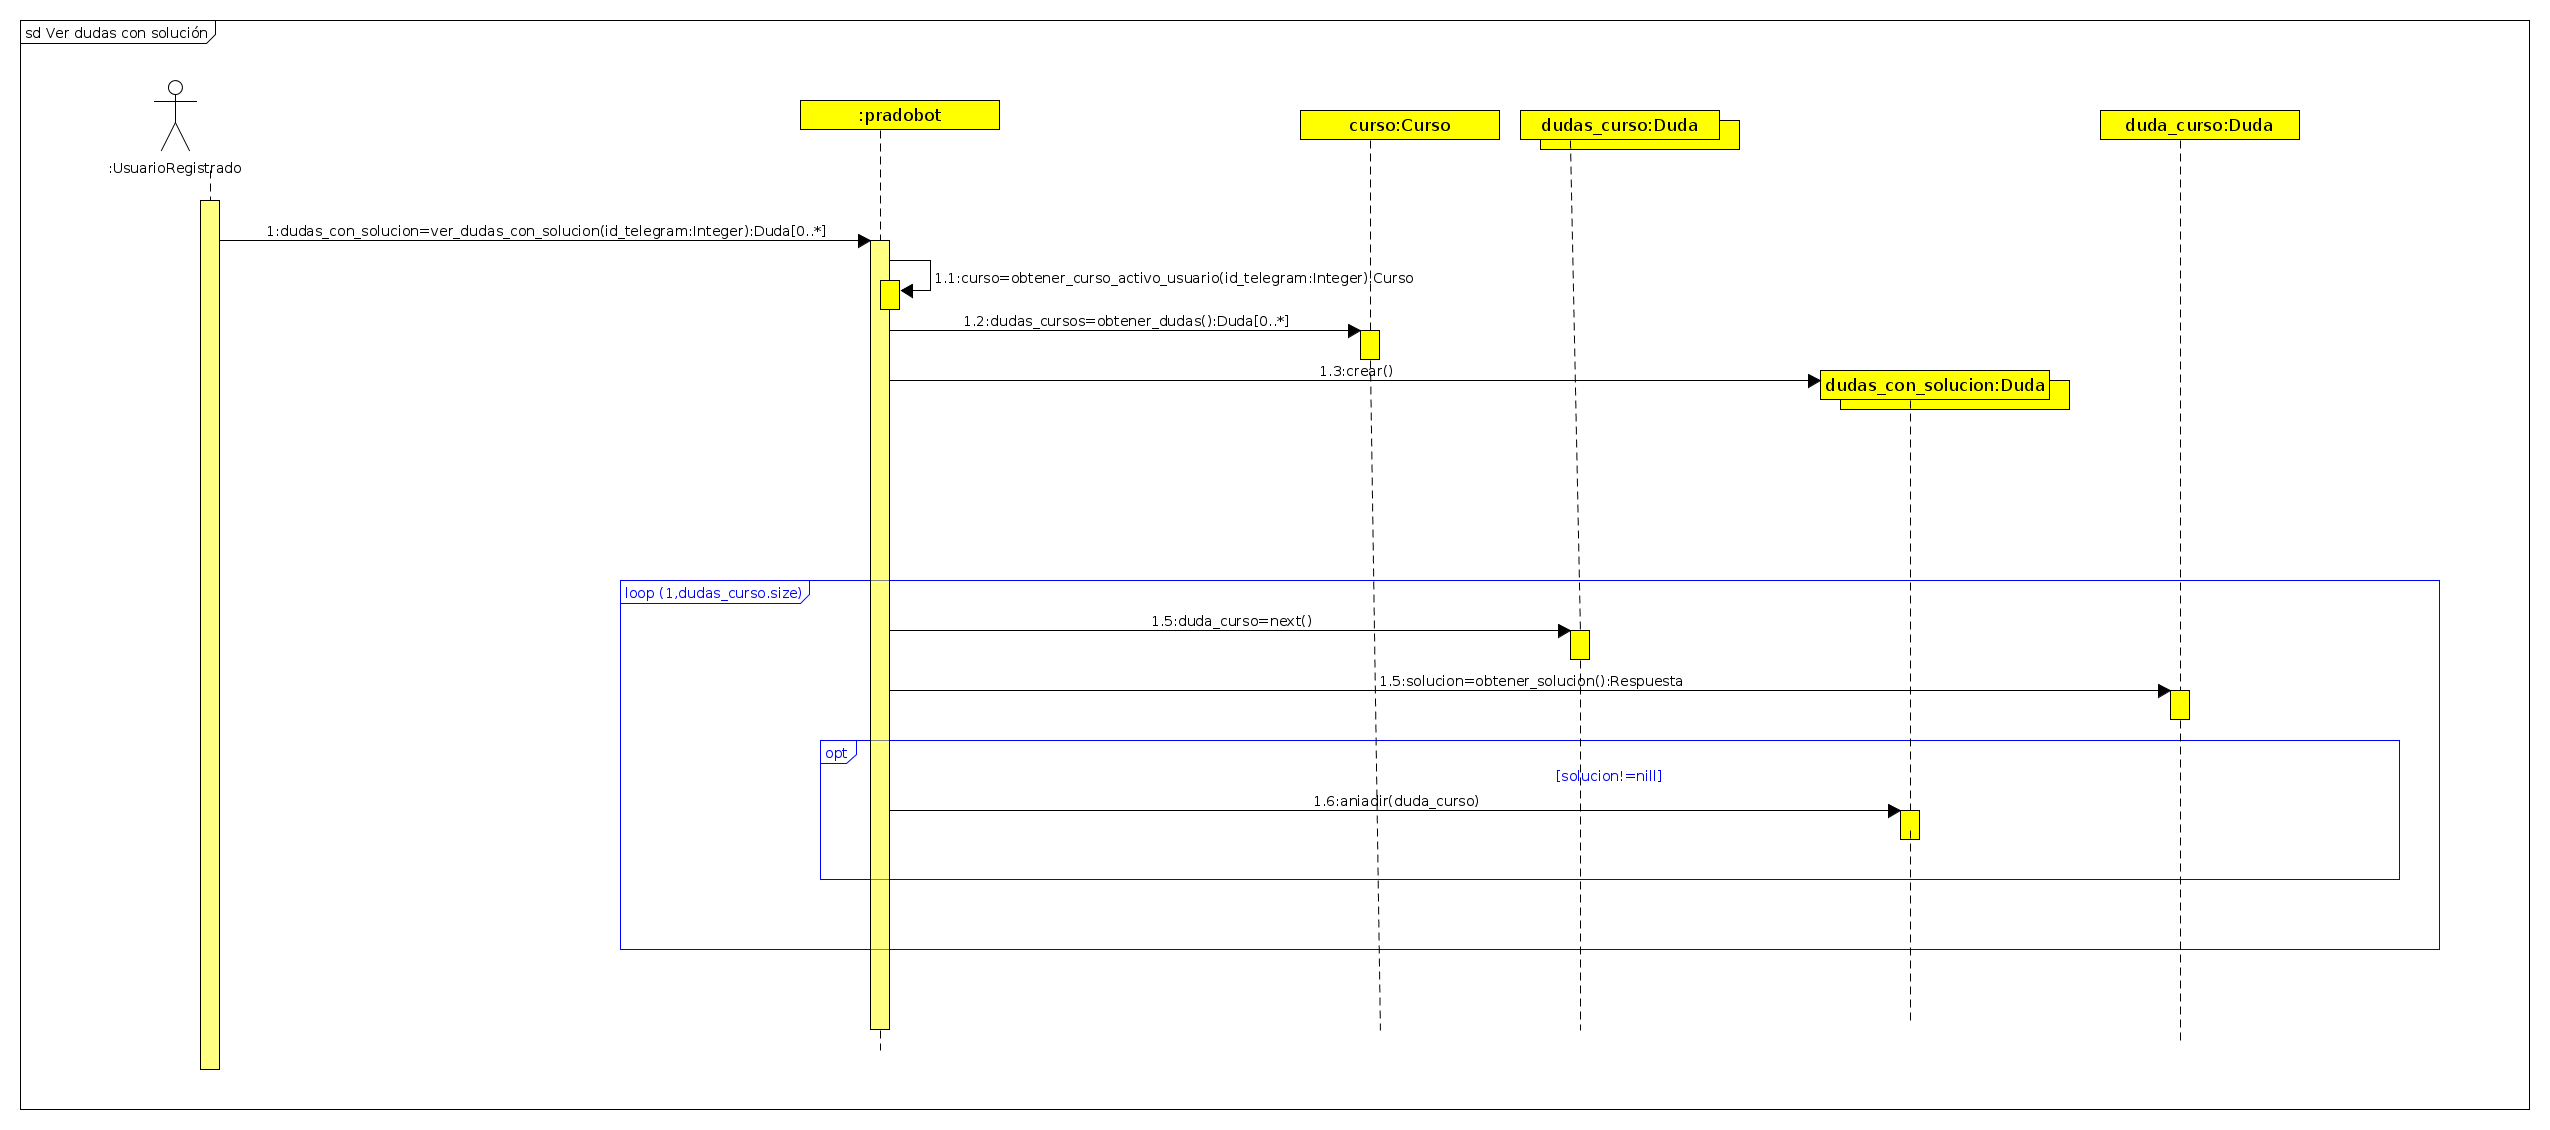
\includegraphics[scale=0.19]{imagenes/diagramas/secuencia/analisis/ver_dudas_resueltas.png}  %el parámetro scale permite agrandar o achicar la imagen. En el nombre de archivo puede especificar directorios

\caption{DS: Ver dudas con solución (CU-5.4) }\label{figura85}

\end{figure}


\begin{figure}[H] %con el [H] le obligamos a situar aquí la figura
\centering
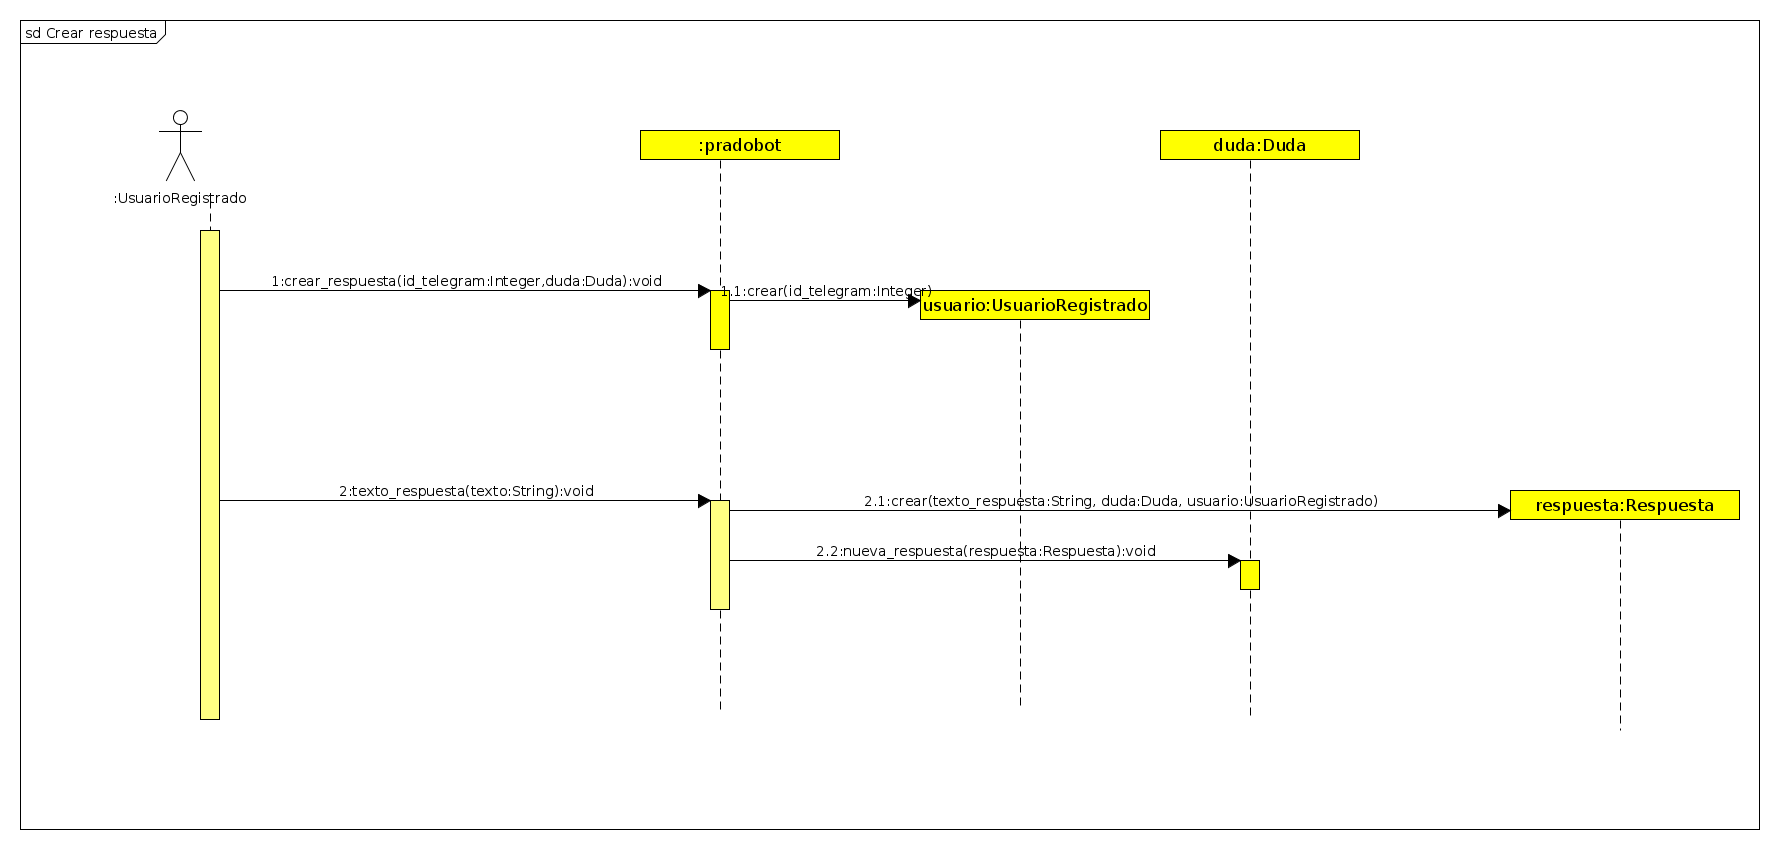
\includegraphics[scale=0.25]{imagenes/diagramas/secuencia/analisis/crear_respuesta.png}  %el parámetro scale permite agrandar o achicar la imagen. En el nombre de archivo puede especificar directorios

\caption{DS: Crear respuesta (CU-5.5) }\label{figura86}

\end{figure}

\begin{figure}[H] %con el [H] le obligamos a situar aquí la figura
\centering
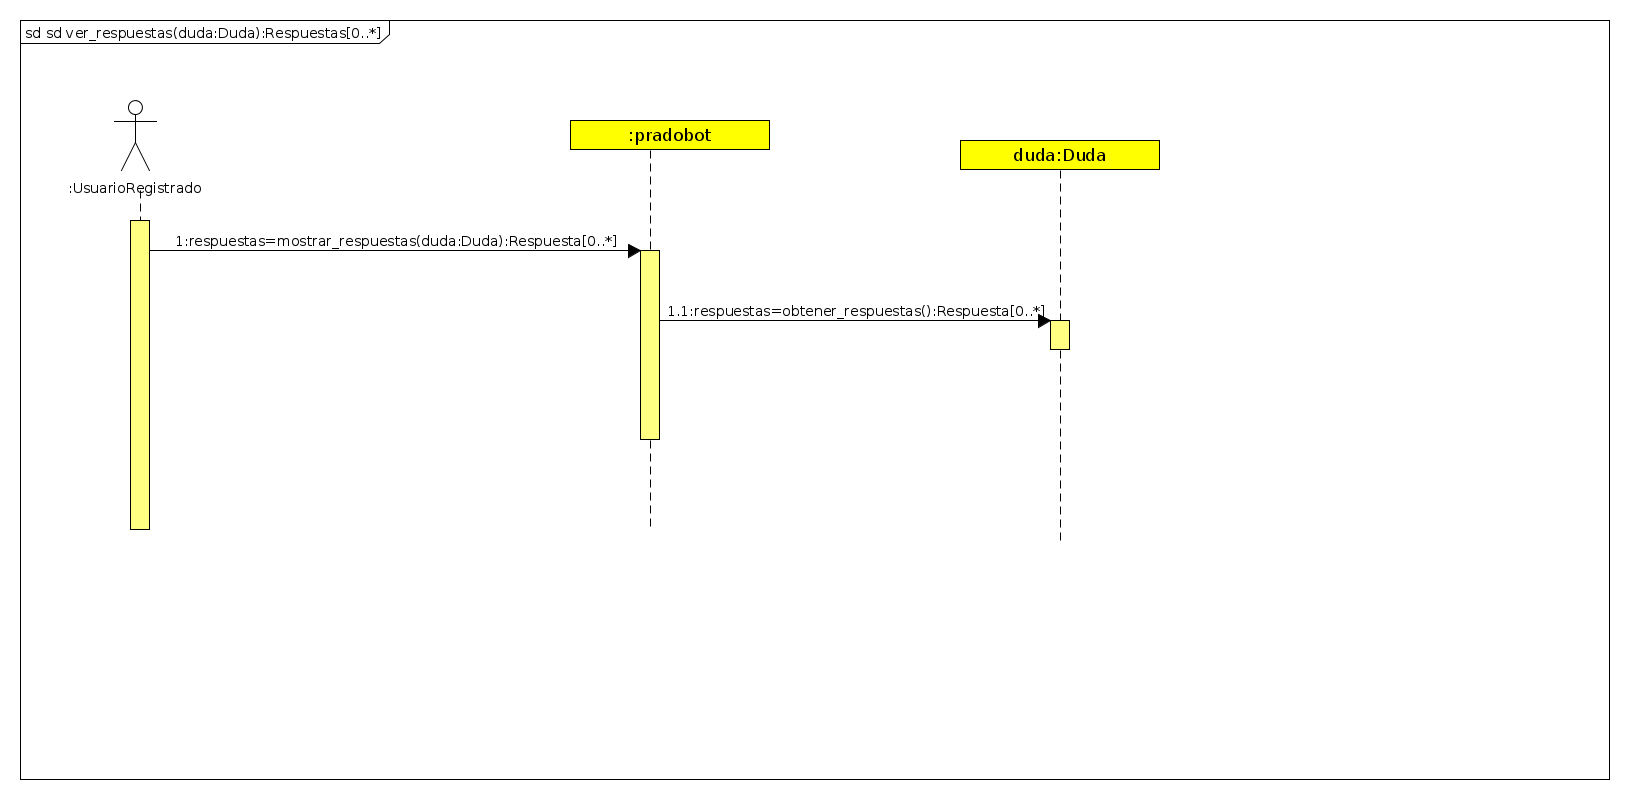
\includegraphics[scale=0.27]{imagenes/diagramas/secuencia/analisis/ver_respuestas_duda.png}  %el parámetro scale permite agrandar o achicar la imagen. En el nombre de archivo puede especificar directorios

\caption{DS: Ver respuestas (CU-5.6) }\label{figura87}

\end{figure}


\begin{figure}[H] %con el [H] le obligamos a situar aquí la figura
\centering
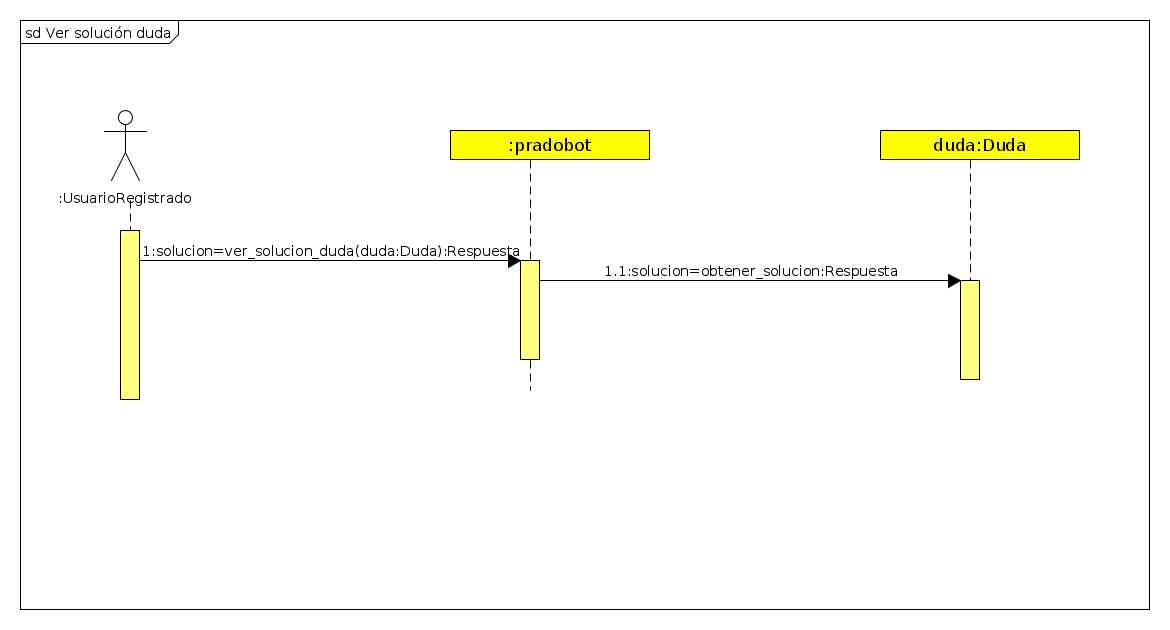
\includegraphics[scale=0.35]{imagenes/diagramas/secuencia/analisis/ver_solucion_duda.png}  %el parámetro scale permite agrandar o achicar la imagen. En el nombre de archivo puede especificar directorios

\caption{DS: Ver solución a duda (CU-5.7) }\label{figura88}

\end{figure}

\begin{figure}[H] %con el [H] le obligamos a situar aquí la figura
\centering
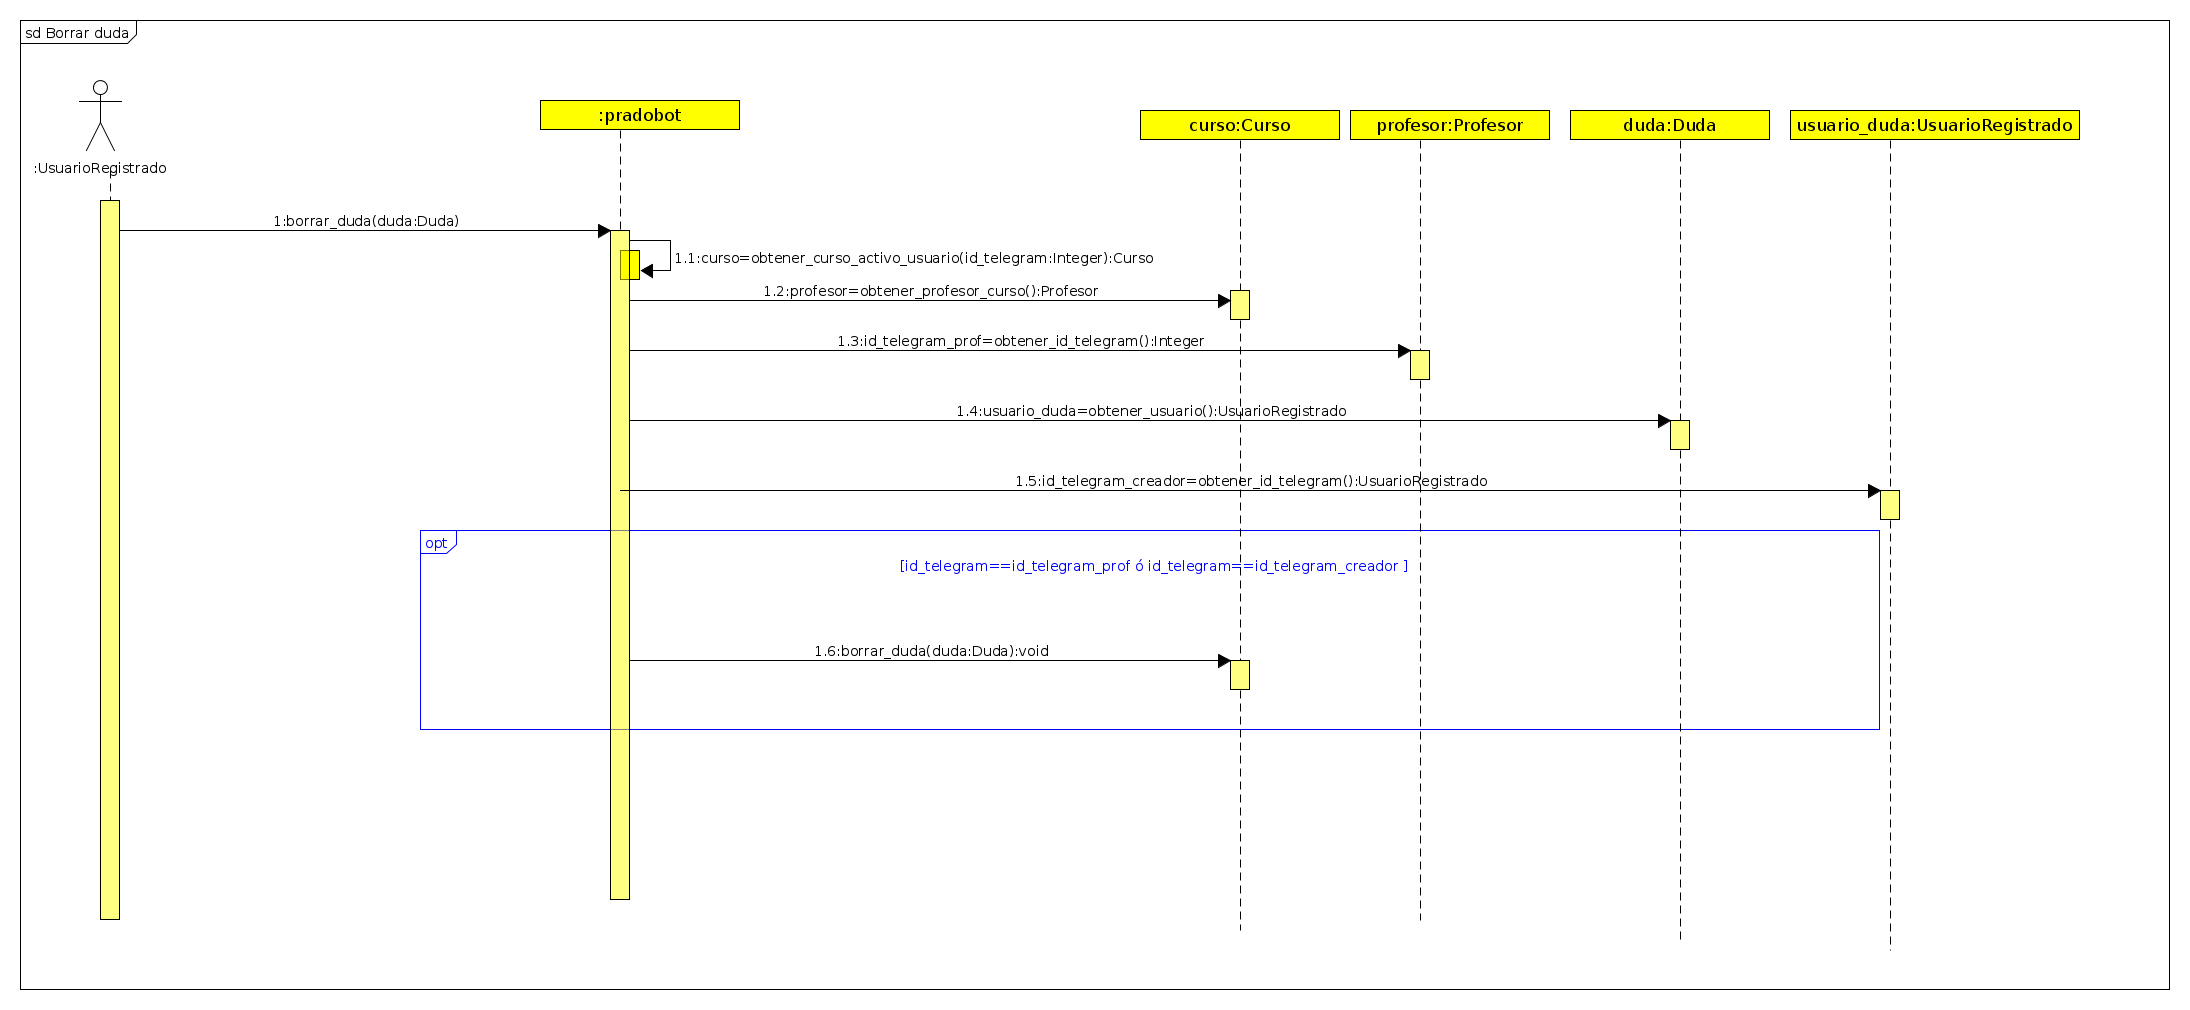
\includegraphics[scale=0.2]{imagenes/diagramas/secuencia/analisis/borrar_duda.png}  %el parámetro scale permite agrandar o achicar la imagen. En el nombre de archivo puede especificar directorios

\caption{DS: Borrar duda (CU-5.8, CU-5.10) }\label{figura89}

\end{figure}

\begin{figure}[H] %con el [H] le obligamos a situar aquí la figura
\centering
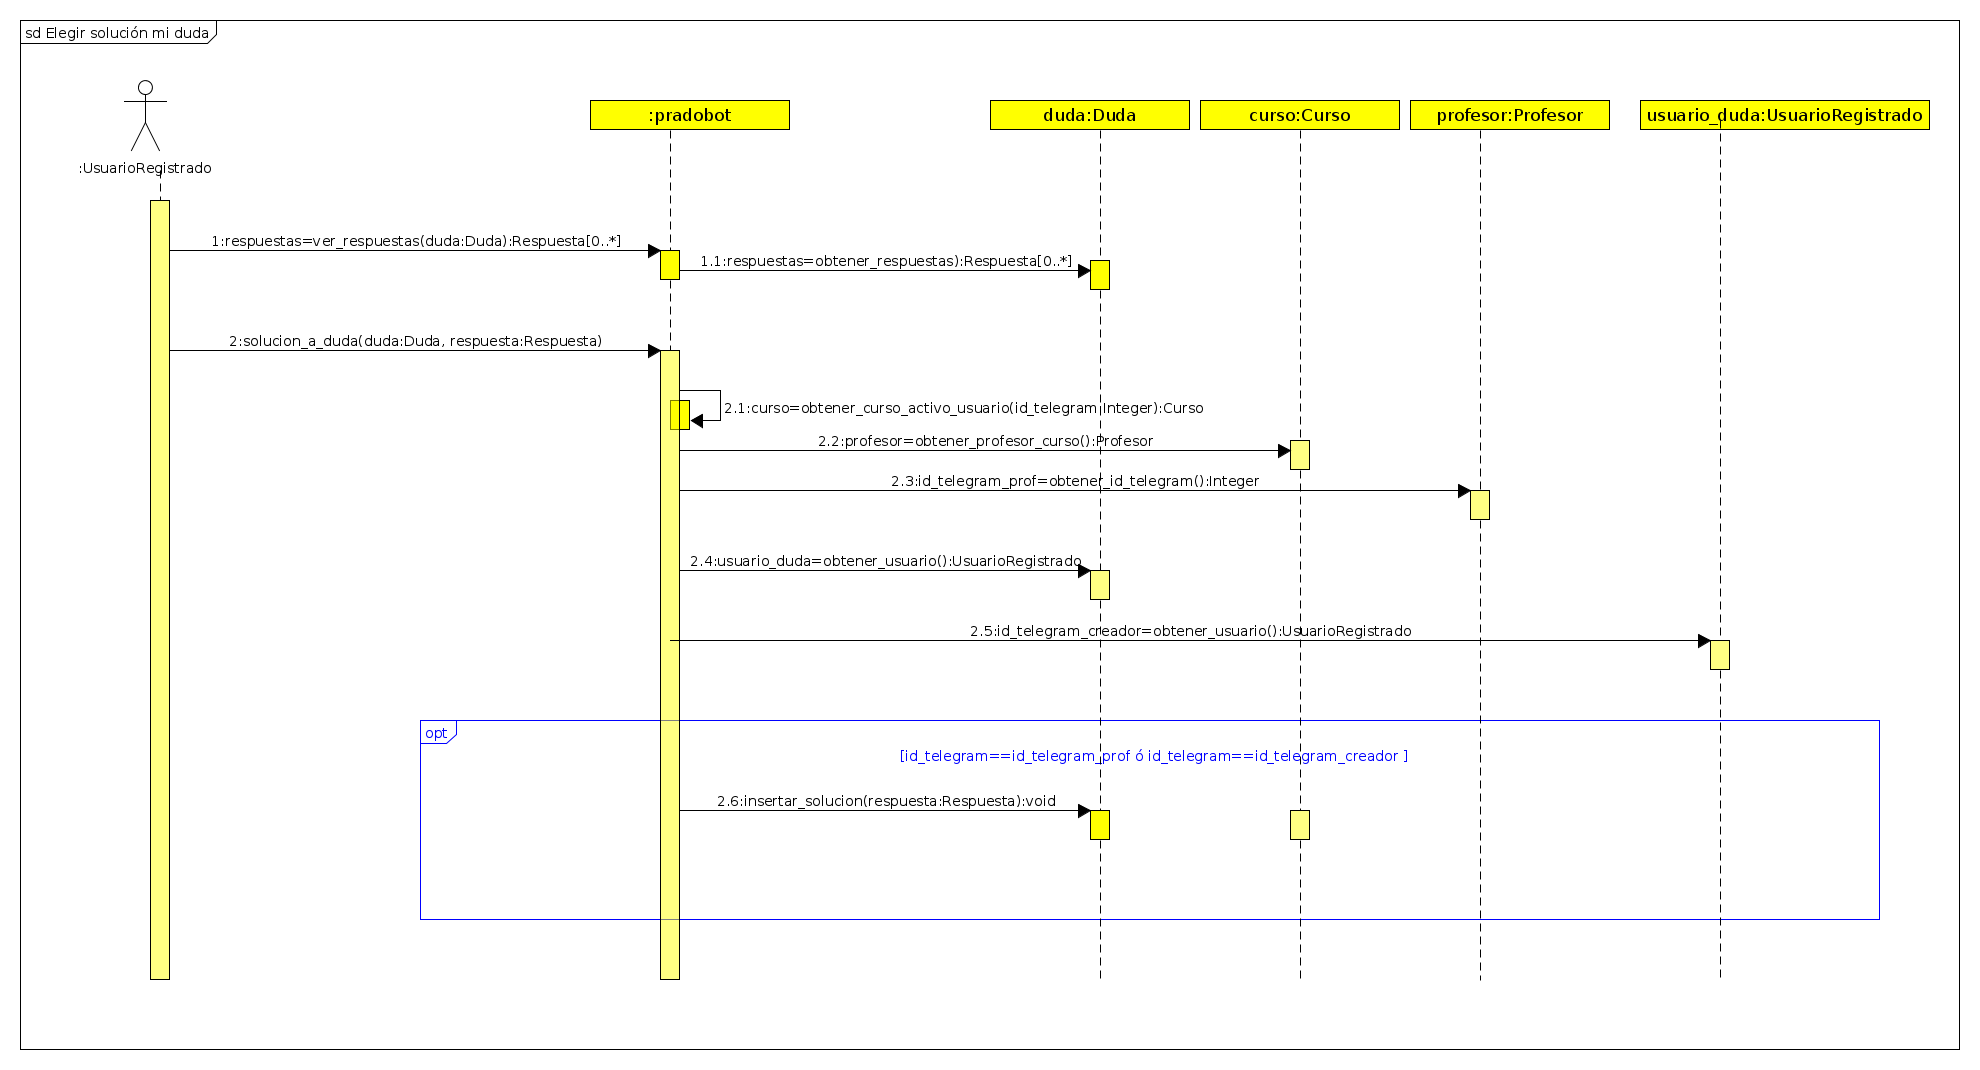
\includegraphics[scale=0.2]{imagenes/diagramas/secuencia/analisis/elegir_solucion_mi_duda.png}  %el parámetro scale permite agrandar o achicar la imagen. En el nombre de archivo puede especificar directorios

\caption{DS: Elegir solución duda (CU-5.9, CU-5.11) }\label{figura90}

\end{figure}


\begin{figure}[H] %con el [H] le obligamos a situar aquí la figura
\centering
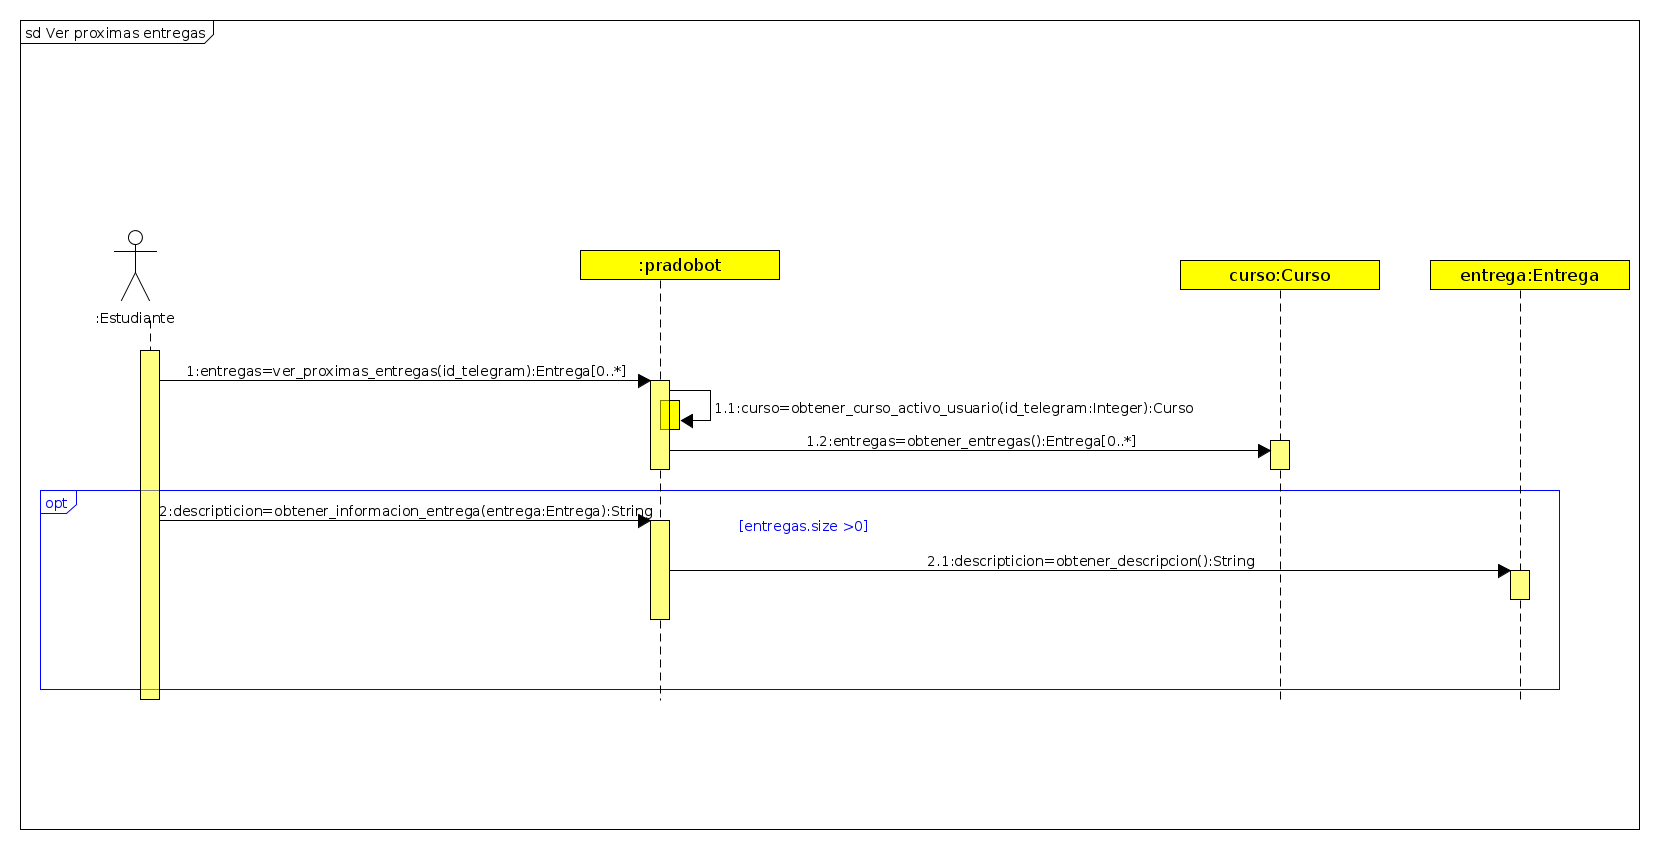
\includegraphics[scale=0.27]{imagenes/diagramas/secuencia/analisis/ver_proximas_entregas.png}  %el parámetro scale permite agrandar o achicar la imagen. En el nombre de archivo puede especificar directorios

\caption{DS: Ver proximas entregas (CU-6.1) }\label{figura91}

\end{figure}


\begin{figure}[H] %con el [H] le obligamos a situar aquí la figura
\centering
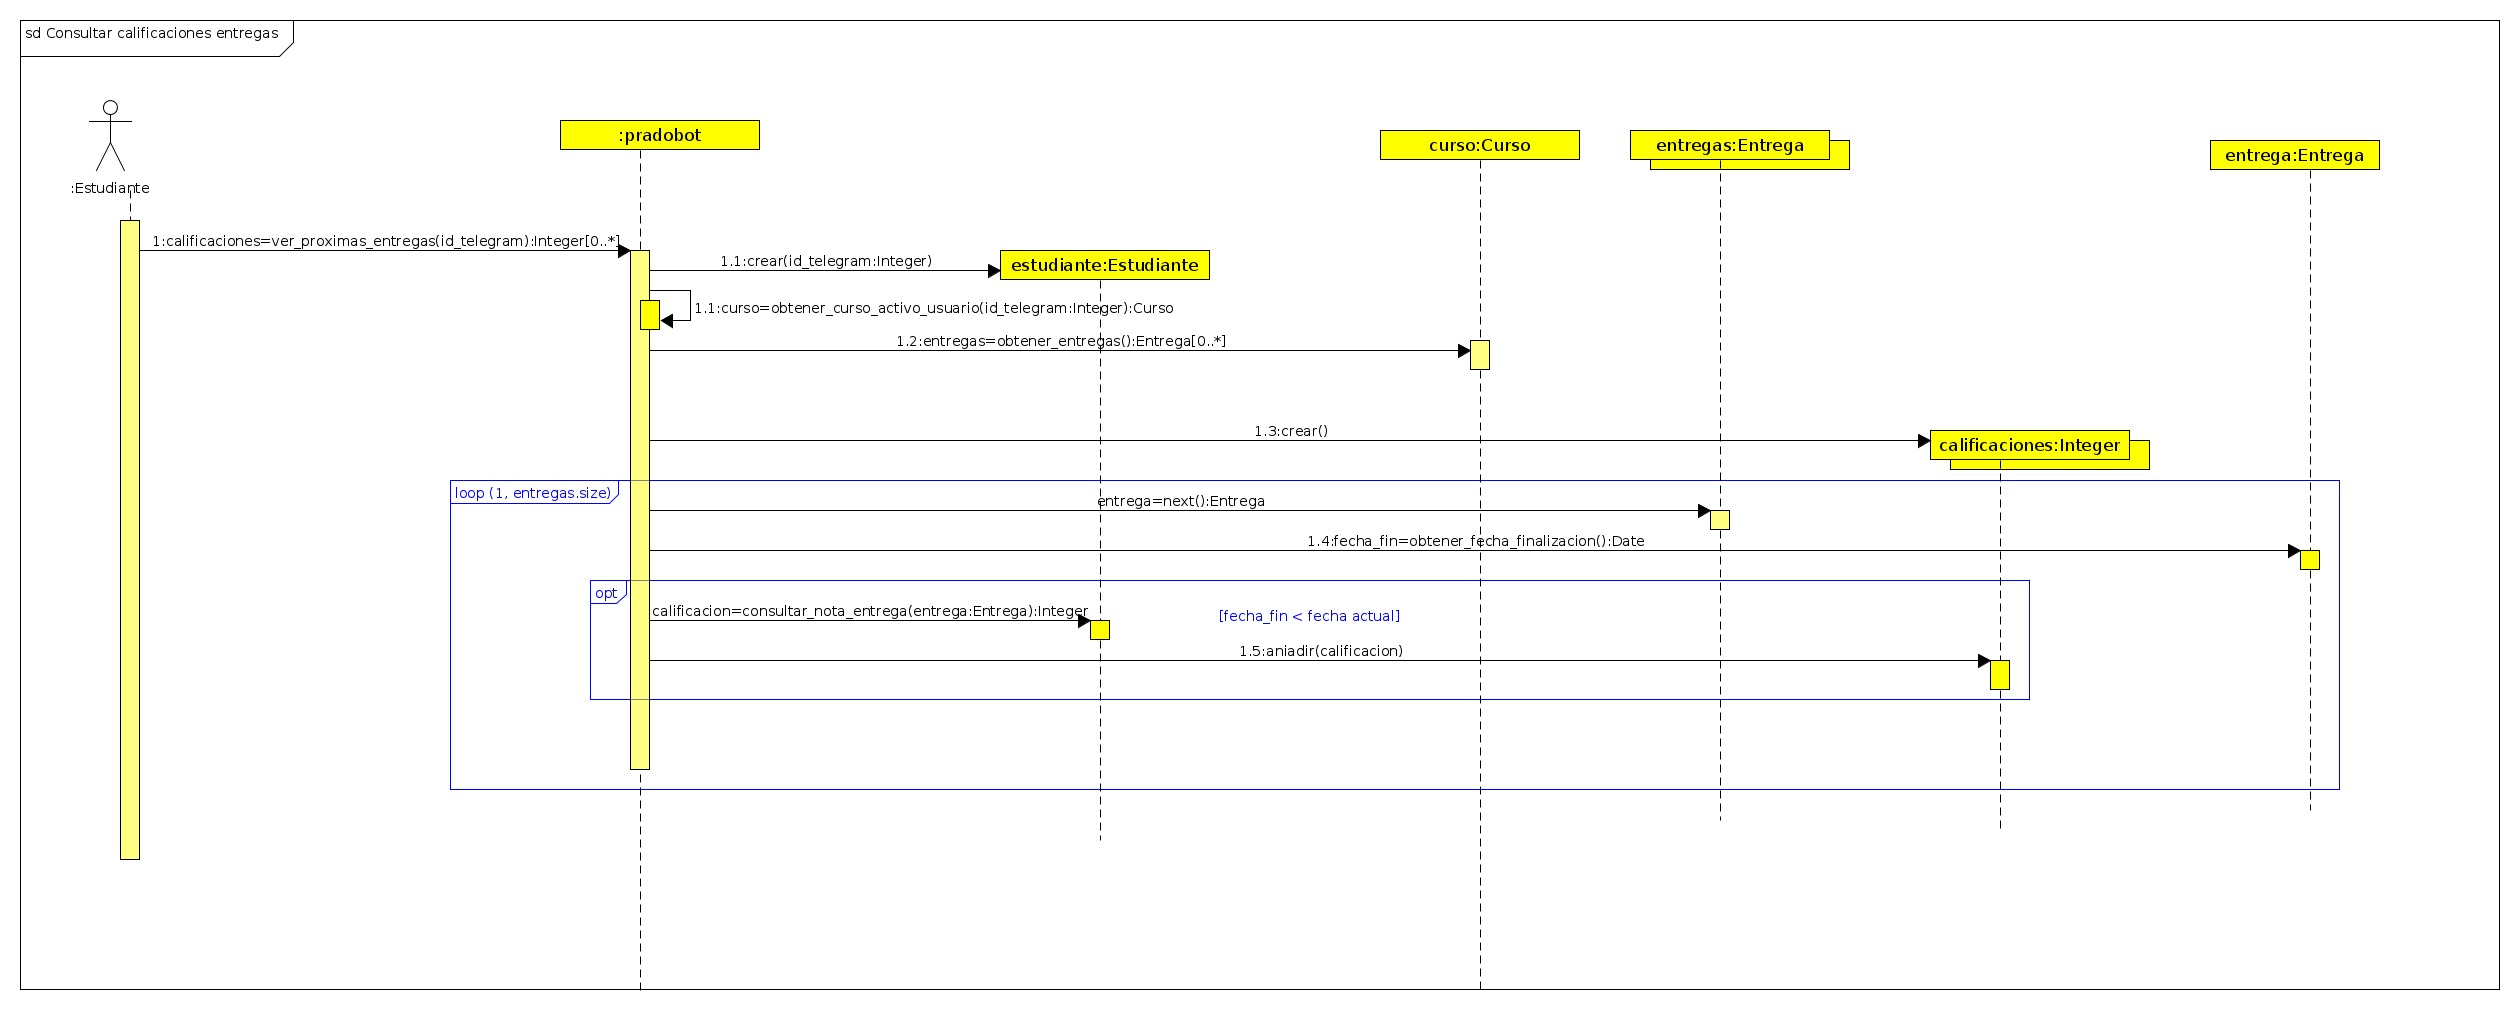
\includegraphics[scale=0.19]{imagenes/diagramas/secuencia/analisis/consultar_calificaciones_entregas.png}  %el parámetro scale permite agrandar o achicar la imagen. En el nombre de archivo puede especificar directorios

\caption{DS: Consultar calificaciones entregas (CU-6.2) }\label{figura92}

\end{figure}




\subsection{Contratos}
    %%%%%%%%%%%%%%%%%%%%%%%%%%%%%%%%%%%%%%%%%%%
   
   
               \begin{table}[!ht]
\begin{tabular}{|c|m{10cm}|}
\hline\rowcolor{Gray}
{\bf Nombre } & {tutorias=obtener\_tutorias()}\\
\hline
{\bf Responsabilidad } & {Obteniene las tutorías de un Profesor.}\\
\hline
\rowcolor{Gray}
{\bf Tipo } & {Profesor} \\
\hline
{\bf Notas } & { } \\
\hline
\rowcolor{Gray}
{\bf Excepciones }& {
\begin{itemize}
\item Que no tenga tutorías el objeto profesor.
\end{itemize}
} \\
\hline
{\bf Salida }& 

	  { 	
	  Para cada objeto tipo Tutoria contenido en tutorias se proporciona:
	  \begin{itemize}
	  \item \enquote{El profesor que la ha creado}
	  \item \enquote{Fecha tutoría}
	  \end{itemize}
	  } 


 \\
\hline
\rowcolor{Gray}
{\bf Precondiciones }& {}\\
\hline
{\bf Poscondiciones }& {
}  \\
\hline
\end{tabular}

\end{table}

 
               \begin{table}[!ht]
\begin{tabular}{|c|m{10cm}|}
\hline\rowcolor{Gray}
{\bf Nombre } & {peticiones=obtener\_peticiones()}\\
\hline
{\bf Responsabilidad } & {Obtiene las peticiones que ha recibido una Tutoria}\\
\hline
\rowcolor{Gray}
{\bf Tipo } & {Tutoria} \\
\hline
{\bf Notas } & { } \\
\hline
\rowcolor{Gray}
{\bf Excepciones }& {
\begin{itemize}
\item Que no haya tenido ninguna petición la tutoría.
\end{itemize}
} \\
\hline
{\bf Salida }& 

	  { 	
	  Para cada objeto Peticion contenido en peticiones se proporciona:
	  \begin{itemize}
	  \item La tutoría a la que se ha realizado la petición
	  \item El estudiante que ha realizado la petición
	  \end{itemize}
	  } 


 \\
\hline
\rowcolor{Gray}
{\bf Precondiciones }& {}\\
\hline
{\bf Poscondiciones }& {
}  \\
\hline
\end{tabular}

\end{table}    
    
    
    
    
    
    
                  \begin{table}[!ht]
\begin{tabular}{|c|m{10cm}|}
\hline\rowcolor{Gray}
{\bf Nombre } & {denegar()}\\
\hline
{\bf Responsabilidad } & {Cambia el estado de  una petición a rechazada}\\
\hline
\rowcolor{Gray}
{\bf Tipo } & {Peticion} \\
\hline
{\bf Notas } & { } \\
\hline
\rowcolor{Gray}
{\bf Excepciones }& {

} \\
\hline
{\bf Salida }& 
	  { 	

	  } 
 \\
\hline
\rowcolor{Gray}
{\bf Precondiciones }& {}\\
\hline
{\bf Poscondiciones }& { Fue modificado el objeto de la clase Peticion cambiándose el valor del atributo estado a \enquote*{rechazada}.
}  \\
\hline
\end{tabular}

\end{table} 
    
    
                      \begin{table}[!ht]
\begin{tabular}{|c|m{10cm}|}
\hline\rowcolor{Gray}
{\bf Nombre } & {aceptar()}\\
\hline
{\bf Responsabilidad } & {Cambia el estado de una Peticion a aceptada}\\
\hline
\rowcolor{Gray}
{\bf Tipo } & {Peticion} \\
\hline
{\bf Notas } & { } \\
\hline
\rowcolor{Gray}
{\bf Excepciones }& {

} \\
\hline
{\bf Salida }& 
	  { 	
	  } 
 \\
\hline
\rowcolor{Gray}
{\bf Precondiciones }& {}\\
\hline
{\bf Poscondiciones }& { El valor del atributo estado del objeto de la clase Peticion fue modificado a \enquote*{aceptada}.
}  \\
\hline
\end{tabular}

\end{table} 


    
                      \begin{table}[!ht]
\begin{tabular}{|c|m{10cm}|}
\hline\rowcolor{Gray}
{\bf Nombre } & {profesor=obtener\_profesor\_curso()}\\
\hline
{\bf Responsabilidad } & {Obteniene a el Profesor responsable de un Curso}\\
\hline
\rowcolor{Gray}
{\bf Tipo } & {Curso} \\
\hline
{\bf Notas } & { } \\
\hline
\rowcolor{Gray}
{\bf Excepciones }& {

} \\
\hline
{\bf Salida }& 
	  { 	
	  Para el objeto profesor de la clase Profesor contenido en profesor se proporciona
	  \begin{itemize}
	  \item id\_telegram
	  \end{itemize}
	  } 
 \\
\hline
\rowcolor{Gray}
{\bf Precondiciones }& {}\\
\hline
{\bf Poscondiciones }& {}.
  \\
\hline
\end{tabular}

\end{table}
 
 
                       \begin{table}[!ht]
\begin{tabular}{|c|m{10cm}|}
\hline\rowcolor{Gray}
{\bf Nombre } & {aceptada=solicitar\_tutoria(peticion)}\\
\hline
{\bf Responsabilidad } & {Realiza una Peticion a una tutoría de un Profesor.}\\
\hline
\rowcolor{Gray}
{\bf Tipo } & {Profesor} \\
\hline
{\bf Notas } & { } \\
\hline
\rowcolor{Gray}
{\bf Excepciones }& {
	  \begin{itemize}
	  \item El estudiante que realiza la petición ya haya realizado otra a la misma tutoría.
	  \item El objeto estudiante de la clase Estudiante contenido en petición no exista.
	  \end{itemize}
} \\
\hline
{\bf Salida }& 
	  { 	
	  Para el objeto aceptada de  la clase Boolean se proporciona el valor true o false.
	  } 
 \\
\hline
\rowcolor{Gray}
{\bf Precondiciones }& {}\\
\hline
{\bf Poscondiciones }& {
\begin{itemize}
\item Fue creado un enlace entre el objeto peticion de la clase Peticion y el objeto de la clase Tutoria
\end{itemize}}
  \\
\hline
\end{tabular}

\end{table}


                       \begin{table}[!ht]
\begin{tabular}{|c|m{10cm}|}
\hline\rowcolor{Gray}
{\bf Nombre } & {id\_telegram=obtener\_telegram()}\\
\hline
{\bf Responsabilidad } & {Obteniene el identificador de Telegram un Profesor}\\
\hline
\rowcolor{Gray}
{\bf Tipo } & {Profesor} \\
\hline
{\bf Notas } & { } \\
\hline
\rowcolor{Gray}
{\bf Excepciones }& {
} \\
\hline
{\bf Salida }& 
	  { 	
	  Devuelve identificador numérico en el objeto de la clase Integer contenido en id\_telegram.
	  } 
 \\
\hline
\rowcolor{Gray}
{\bf Precondiciones }& {}\\
\hline
{\bf Poscondiciones }& {}.
  \\
\hline
\end{tabular}

\end{table}



                       \begin{table}[!ht]
\begin{tabular}{|c|m{10cm}|}
\hline\rowcolor{Gray}
{\bf Nombre } & {usuario\_duda=obtener\_usuario()}\\
\hline
{\bf Responsabilidad } & {Obteniene al UsuarioRegistrado creador de una Duda}\\
\hline
\rowcolor{Gray}
{\bf Tipo } & {Profesor} \\
\hline
{\bf Notas } & { } \\
\hline
\rowcolor{Gray}
{\bf Excepciones }& {
} \\
\hline
{\bf Salida }& 
	  { 	
	  Para el objeto UsuarioRegistrado contenido en usuario\_duda se proporciona:
	  \begin{itemize}
	  \item id\_telegram
	  \end{itemize}
	  } 
 \\
\hline
\rowcolor{Gray}
{\bf Precondiciones }& {}\\
\hline
{\bf Poscondiciones }& {}.
  \\
\hline
\end{tabular}

\end{table}



                       \begin{table}[!ht]
\begin{tabular}{|c|m{10cm}|}
\hline\rowcolor{Gray}
{\bf Nombre } & {id\_telegram=obtener\_telegram()}\\
\hline
{\bf Responsabilidad } & {Obtiene el identificador numérico de un UsuarioRegistrado}\\
\hline
\rowcolor{Gray}
{\bf Tipo } & {UsuarioRegistrado} \\
\hline
{\bf Notas } & { } \\
\hline
\rowcolor{Gray}
{\bf Excepciones }& {
} \\
\hline
{\bf Salida }& 
	  { 	
	  Devuelve identificador numérico para el objeto id\_telegram de la clase Integer.
	  } 
 \\
\hline
\rowcolor{Gray}
{\bf Precondiciones }& {}\\
\hline
{\bf Poscondiciones }& {}
  \\
\hline
\end{tabular}

\end{table}



                       \begin{table}[!ht]
\begin{tabular}{|c|m{10cm}|}
\hline\rowcolor{Gray}
{\bf Nombre } & {borrar\_duda(duda)}\\
\hline
{\bf Responsabilidad } & {Borra una Duda de un Curso}\\
\hline
\rowcolor{Gray}
{\bf Tipo } & {Curso} \\
\hline
{\bf Notas } & { } \\
\hline
\rowcolor{Gray}
{\bf Excepciones }& {
\begin{itemize}
\item Que no exista el objeto duda de la clase Duda.
\end{itemize}
} \\
\hline
{\bf Salida }& 
	  { 	
	  } 
 \\
\hline
\rowcolor{Gray}
{\bf Precondiciones }& {
}\\
\hline
{\bf Poscondiciones }& {

\begin{itemize}
\item Fue borrado el enlace entre el objeto duda y el el objeto de la clase Curso .
\item Para cada objeto r de la clase Respuesta relacionado con el objeto duda de la clase Duda:
\begin{itemize}
\item Fue borrado el enlace entre r y duda.
\item Fue borrado el objeto r.
\end{itemize}
\item Fue borrado el enlace entre duda y el objeto de clase UsuarioRegistrado relacionado con duda.
\item Fue borrado el objeto duda.
\end{itemize}

}.
 \\
\hline
\end{tabular}

\end{table}

                       \begin{table}[!ht]
\begin{tabular}{|c|m{10cm}|}
\hline\rowcolor{Gray}
{\bf Nombre } & {borrar\_tutoria(tutoria)}\\
\hline
{\bf Responsabilidad } & {Elimina una Tutoria de un Profesor}\\
\hline
\rowcolor{Gray}
{\bf Tipo } & {Profesor} \\
\hline
{\bf Notas } & { } \\
\hline
\rowcolor{Gray}
{\bf Excepciones }& {
\begin{itemize}
\item Que no exista el objeto tutoria de la clase Tutoria.
\end{itemize}
} \\
\hline
{\bf Salida }& 
	  { 	
	  } 
 \\
\hline
\rowcolor{Gray}
{\bf Precondiciones }& {
}\\
\hline
{\bf Poscondiciones }& {

\begin{itemize}
\item Fue borrado el enlace entre el objeto tutoria y el el objeto de la clase Profesor .
\item Para cada objeto p de la clase Petición relacionado con el objeto tutoria de la clase Tutoria:
\begin{itemize}
\item Fue borrado el enlace entre p y tutoria.
\item Fue borrado el enlace entre p y el objeto de la clase Estudiante con el que está relacionado.
\item Fue borrado el objeto p.
\end{itemize}
\item Fue borrado el objeto tutoria
\end{itemize}

}.
  \\
\hline
\end{tabular}

\end{table}


                       \begin{table}[!ht]
\begin{tabular}{|c|m{10cm}|}
\hline\rowcolor{Gray}
{\bf Nombre } & {entregas=obtener\_entregas()}\\
\hline
{\bf Responsabilidad } & {Obtener las entregas de un Curso}\\
\hline
\rowcolor{Gray}
{\bf Tipo } & {Profesor} \\
\hline
{\bf Notas } & { } \\
\hline
\rowcolor{Gray}
{\bf Excepciones }& {
\begin{itemize}
\item No tenga ninguna entrega el objeto de la clase Curso.
\end{itemize}
} \\
\hline
{\bf Salida }& 
	  { 	
	  Para cada objeto Entrega contenido en entregas se proporciona:
	  \begin{itemize}
	  \item fecha\_fin
	  \item identificador
	  \item nombre
	  \end{itemize}	  } 
 \\
\hline
\rowcolor{Gray}
{\bf Precondiciones }& {
}\\
\hline
{\bf Poscondiciones }& {
}
  \\
\hline
\end{tabular}

\end{table}




                       \begin{table}[!ht]
\begin{tabular}{|c|m{10cm}|}
\hline\rowcolor{Gray}
{\bf Nombre } & {fecha\_fin=obtener\_fecha\_finalizacion()}\\
\hline
{\bf Responsabilidad } & {Obteniene la fecha finalización de una Entrega}\\
\hline
\rowcolor{Gray}
{\bf Tipo } & {Entrega} \\
\hline
{\bf Notas } & { } \\
\hline
\rowcolor{Gray}
{\bf Excepciones }& {
} \\
\hline
{\bf Salida }& 
	  { 	
	  Se devuelve el valor del atributo fecha\_fin del objeto de la clase Entrega en el objeto tipo Date contenido en fecha\_fin } 
 \\
\hline
\rowcolor{Gray}
{\bf Precondiciones }& {
}\\
\hline
{\bf Poscondiciones }& {
}
  \\
\hline
\end{tabular}

\end{table}




                       \begin{table}[!ht]
\begin{tabular}{|c|m{10cm}|}
\hline\rowcolor{Gray}
{\bf Nombre } & {aniadir\_duda(duda)}\\
\hline
{\bf Responsabilidad } & {Añade una nueva Duda al Curso}\\
\hline
\rowcolor{Gray}
{\bf Tipo } & {Curso} \\
\hline
{\bf Notas } & { } \\
\hline
\rowcolor{Gray}
{\bf Excepciones }& {
} \\
\hline
{\bf Salida }& 
	  { 	
 } 
 \\
\hline
\rowcolor{Gray}
{\bf Precondiciones }& {
}\\
\hline
{\bf Poscondiciones }& {
\begin{itemize}
\item Fue creado un enlace entre el objeto duda de la clase Duda y el objeto de la clase Curso.
\end{itemize}
}
  \\
\hline
\end{tabular}

\end{table}








                       \begin{table}[!ht]
\begin{tabular}{|c|m{10cm}|}
\hline\rowcolor{Gray}
{\bf Nombre } & {nueva\_respuesta(respuesta)}\\
\hline
{\bf Responsabilidad } & {Añade una nueva Respuesta a una Duda}\\
\hline
\rowcolor{Gray}
{\bf Tipo } & {Duda} \\
\hline
{\bf Notas } & { } \\
\hline
\rowcolor{Gray}
{\bf Excepciones }& {
} \\
\hline
{\bf Salida }& 
	  { 	
} 
 \\
\hline
\rowcolor{Gray}
{\bf Precondiciones }& {
}\\
\hline
{\bf Poscondiciones }& { Fue creado un enlace entre el objeto respuesta de la clase Respuesta y el objeto de la clase Duda.
}
  \\
\hline
\end{tabular}

\end{table}






                       \begin{table}[!ht]
\begin{tabular}{|c|m{10cm}|}
\hline\rowcolor{Gray}
{\bf Nombre } & {cursos=obtener\_cursos()}\\
\hline
{\bf Responsabilidad } & {Obtiene los cursos en los que está dado de alta un UsuarioRegistrado}\\
\hline
\rowcolor{Gray}
{\bf Tipo } & {UsuarioRegistrado} \\
\hline
{\bf Notas } & { } \\
\hline
\rowcolor{Gray}
{\bf Excepciones }& {
} \\
\hline
{\bf Salida }& 
	  {
Para cada objeto Curso contenido en cursos se proporciona:	  
	   	\begin{itemize}
	  \item id\_curso
	  \item nombre\_curso
	    \end{itemize}
} 
 \\
\hline
\rowcolor{Gray}
{\bf Precondiciones }& {
}\\
\hline
{\bf Poscondiciones }& { }
  \\
\hline
\end{tabular}

\end{table}





                       \begin{table}[!ht]
\begin{tabular}{|c|m{10cm}|}
\hline\rowcolor{Gray}
{\bf Nombre } & {respuestas=obtener\_respuestas()}\\
\hline
{\bf Responsabilidad } & {Obtiene las respuestas que tiene una Duda}\\
\hline
\rowcolor{Gray}
{\bf Tipo } & {Duda} \\
\hline
{\bf Notas } & { } \\
\hline
\rowcolor{Gray}
{\bf Excepciones }& {
\begin{itemize}
\item Que no haya tenido ninguna respuesta la duda.
\end{itemize}
} \\
\hline
{\bf Salida }& 
	  {
Para cada objeto Respuesta contenido en respuestas se proporciona:	  
	   	\begin{itemize}
	  \item contenido
	  \item usuario
	  \item duda
	    \end{itemize}
} 
 \\
\hline
\rowcolor{Gray}
{\bf Precondiciones }& {
}\\
\hline
{\bf Poscondiciones }& { }
  \\
\hline
\end{tabular}

\end{table}





\clearpage

                       \begin{table}[!ht]
\begin{tabular}{|c|m{10cm}|}
\hline\rowcolor{Gray}
{\bf Nombre } & {insertar\_solucion(respuesta:Respuesta)}\\
\hline
{\bf Responsabilidad } & {Asigna una Respuesta como solución a una Duda}\\
\hline
\rowcolor{Gray}
{\bf Tipo } & {Duda} \\
\hline
{\bf Notas } & { } \\
\hline
\rowcolor{Gray}
{\bf Excepciones }& {
	   	\begin{itemize}
	  \item El objeto Duda ya tenga solución.
	    \end{itemize}
} \\
\hline
{\bf Salida }& 
	  {
} 
 \\
\hline
\rowcolor{Gray}
{\bf Precondiciones }& {
}\\
\hline
{\bf Poscondiciones }& { 
Fue creado un nuevo enlace entre el objeto respuesta de la clase Respuesta y el objeto de la clase Duda.}	  
  \\
\hline
\end{tabular}

\end{table}

\clearpage

                       \begin{table}[!ht]
\begin{tabular}{|c|m{10cm}|}
\hline\rowcolor{Gray}
{\bf Nombre } & {solucion=obtener\_solucion())}\\
\hline
{\bf Responsabilidad } & {Obtiene el objeto Respuesta que resuelve una Duda}\\
\hline
\rowcolor{Gray}
{\bf Tipo } & {Duda} \\
\hline
{\bf Notas } & { } \\
\hline
\rowcolor{Gray}
{\bf Excepciones }& {
	   	\begin{itemize}
	  \item Objeto de la clase Duda no tenga ningún objeto de la clase Respuesta que sea su solución.
	    \end{itemize}
} \\
\hline
{\bf Salida }& 
	  { Para el objeto de la clase Respuesta contenido en respuesta  se proporciona:
	   	\begin{itemize}
	  \item contenido
	  \item usuario
	  \item duda
	    \end{itemize}
} 
 \\
\hline
\rowcolor{Gray}
{\bf Precondiciones }& {
}\\
\hline
{\bf Poscondiciones }& { 
  }
  \\
\hline
\end{tabular}

\end{table}


                       \begin{table}[!ht]
\begin{tabular}{|c|m{10cm}|}
\hline\rowcolor{Gray}
{\bf Nombre } & {dudas\_curso=obtener\_dudas())}\\
\hline
{\bf Responsabilidad } & {Obtiene las dudas asociadas a un Curso}\\
\hline
\rowcolor{Gray}
{\bf Tipo } & {Curso} \\
\hline
{\bf Notas } & { } \\
\hline
\rowcolor{Gray}
{\bf Excepciones }& {
	   	\begin{itemize}
	  \item Que el objeto Curso no tenga ninguna duda asociada.
	    \end{itemize}
} \\
\hline
{\bf Salida }& 
	  { Para cada objeto Duda contenido en dudas se proporciona:
	   	\begin{itemize}
	  \item contenido
	  \item usuario
	  	    \end{itemize}
} 
 \\
\hline
\rowcolor{Gray}
{\bf Precondiciones }& {
}\\
\hline
{\bf Poscondiciones }& { 
  }
  \\
\hline
\end{tabular}

\end{table}






                       \begin{table}[!ht]
\begin{tabular}{|c|m{10cm}|}
\hline\rowcolor{Gray}
{\bf Nombre } & {estado=obtener\_estado())}\\
\hline
{\bf Responsabilidad } & {Obtiene el estado de una Peticion}\\
\hline
\rowcolor{Gray}
{\bf Tipo } & {Peticion} \\
\hline
{\bf Notas } & { } \\
\hline
\rowcolor{Gray}
{\bf Excepciones }& {
} \\
\hline
{\bf Salida }& 
	  { Se proporciona el valor del atributo estado de un objeto de la clase Peticion  en el objeto estado de la clase String.
} 
 \\
\hline
\rowcolor{Gray}
{\bf Precondiciones }& {
}\\
\hline
{\bf Poscondiciones }& { 
  }
  \\
\hline
\end{tabular}

\end{table}



                       \begin{table}[!ht]
\begin{tabular}{|c|m{10cm}|}
\hline\rowcolor{Gray}
{\bf Nombre } & {fecha=obtener\_fecha())}\\
\hline
{\bf Responsabilidad } & {Proporciona la fecha que tiene una Tutoria.}\\
\hline
\rowcolor{Gray}
{\bf Tipo } & {Tutoria} \\
\hline
{\bf Notas } & { } \\
\hline
\rowcolor{Gray}
{\bf Excepciones }& {
} \\
\hline
{\bf Salida }& 
	  { Se proporciona el valor del atributo fecha de un objeto de la clase Tutoria  en el objeto fecha de la clase Date.
} 
 \\
\hline
\rowcolor{Gray}
{\bf Precondiciones }& {
}\\
\hline
{\bf Poscondiciones }& { 
  }
  \\
\hline
\end{tabular}

\end{table}





                       \begin{table}[!ht]
\begin{tabular}{|c|m{10cm}|}
\hline\rowcolor{Gray}
{\bf Nombre } & {dudas=obtener\_dudas())}\\
\hline
{\bf Responsabilidad } & {Obtiene las dudas creadas por un UsuarioRegistrado}\\
\hline
\rowcolor{Gray}
{\bf Tipo } & {UsuarioRegistrado} \\
\hline
{\bf Notas } & { } \\
\hline
\rowcolor{Gray}
{\bf Excepciones }& {
} \\
\hline
{\bf Salida }& 
	  { Para cada objeto de la clase duda contenido en dudas se proporciona:
	  \begin{itemize}
	  \item contenido
	  \item usuario
	  \end{itemize}
} 
 \\
\hline
\rowcolor{Gray}
{\bf Precondiciones }& {
}\\
\hline
{\bf Poscondiciones }& { 
  }
  \\
\hline
\end{tabular}

\end{table}





                       \begin{table}[!ht]
\begin{tabular}{|c|m{10cm}|}
\hline\rowcolor{Gray}
{\bf Nombre } & {peticiones=obtener\_peticiones\_tutoria())}\\
\hline
{\bf Responsabilidad } & {Obtiene las peticiones realizadas por un Estudiante a una Tutoria}\\
\hline
\rowcolor{Gray}
{\bf Tipo } & {Estudiante} \\
\hline
{\bf Notas } & { } \\
\hline
\rowcolor{Gray}
{\bf Excepciones }& {
\begin{itemize}
\item El estudiante no haya realizado ninguna petición a una tutoría del profesor.
\end{itemize}

} \\
\hline
{\bf Salida }& 
	  { Para cada objeto Peticion contenido en peticiones se proporciona:
	  \begin{itemize}
	  \item tutoria
	  \item estudiante
	  \item hora
	  \end{itemize}
} 
 \\
\hline
\rowcolor{Gray}
{\bf Precondiciones }& {
}\\
\hline
{\bf Poscondiciones }& { 
  }
  \\
\hline
\end{tabular}

\end{table}







                       \begin{table}[!ht]
\begin{tabular}{|c|m{10cm}|}
\hline\rowcolor{Gray}
{\bf Nombre } & {descripcion=obtener\_descripcion())}\\
\hline
{\bf Responsabilidad } & {Obtiene la descripción de una entrega.}\\
\hline
\rowcolor{Gray}
{\bf Tipo } & {Estudiante} \\
\hline
{\bf Notas } & { } \\
\hline
\rowcolor{Gray}
{\bf Excepciones }& {
\begin{itemize}
\item La entrega no tenga descripcion.
\end{itemize}
} \\
\hline
{\bf Salida }& 
	  { Se proporciona el valor del atributo descripción del objeto de la clase entrega en el objeto descripcion de la clase String.
} 
 \\
\hline
\rowcolor{Gray}
{\bf Precondiciones }& {
}\\
\hline
{\bf Poscondiciones }& { 
  }
  \\
\hline
\end{tabular}

\end{table}




                       \begin{table}[!ht]
\begin{tabular}{|c|m{10cm}|}
\hline\rowcolor{Gray}
{\bf Nombre } & {establecer\_nueva\_tutoria(tutoria))}\\
\hline
{\bf Responsabilidad } & {Crea una nueva tutoría para el profesor}\\
\hline
\rowcolor{Gray}
{\bf Tipo } & {UsuarioRegistrado} \\
\hline
{\bf Notas } & { } \\
\hline
\rowcolor{Gray}
{\bf Excepciones }& {
	   	\begin{itemize}
	  \item Objeto de la clase Tutoria con los mismos datos ya exista.
	    \end{itemize}
} \\
\hline
{\bf Salida }& 
	  {
} 
 \\
\hline
\rowcolor{Gray}
{\bf Precondiciones }& {
}\\
\hline
{\bf Poscondiciones }& { 
Fue creado un enlace entre el objeto tutoria de la clase tutoria y el objeto de la clase Profesor.	  }
  \\
\hline
\end{tabular}

\end{table}



                       \begin{table}[!ht]
\begin{tabular}{|c|m{10cm}|}
\hline\rowcolor{Gray}
{\bf Nombre } & {establecer\_nueva\_tutoria(tutoria))}\\
\hline
{\bf Responsabilidad } & {Crea una nueva tutoría para el profesor}\\
\hline
\rowcolor{Gray}
{\bf Tipo } & {UsuarioRegistrado} \\
\hline
{\bf Notas } & { } \\
\hline
\rowcolor{Gray}
{\bf Excepciones }& {
	   	\begin{itemize}
	  \item Objeto de la clase Tutoria con los mismos datos ya exista.
	    \end{itemize}
} \\
\hline
{\bf Salida }& 
	  {
} 
 \\
\hline
\rowcolor{Gray}
{\bf Precondiciones }& {
}\\
\hline
{\bf Poscondiciones }& { 
Fue creado un enlace entre el objeto tutoria de la clase tutoria y el objeto de la clase Profesor.	  }
  \\
\hline
\end{tabular}

\end{table}

\clearpage